\documentclass[12pt]{article}
%\usepackage[margin=0.25in]{geometry}
\usepackage[margin=1.0in]{geometry}
\usepackage{graphicx}
\usepackage{color}
\usepackage{xcolor}
\usepackage{hyperref}
\usepackage{amsmath}
\usepackage{enumitem}
%\setlist[1]{itemsep=-2pt}
\usepackage{mdwlist}

\definecolor{myBlue}{rgb}{0.2,0.2,0.6}
\definecolor{myGreen}{rgb}{0.0,0.26,0.15}
\definecolor{om}{rgb}{0.4,0.19,0.28} % om - old mauve

\setlength{\parindent}{0em}
\setlength{\parskip}{0.5em}

\title{\vspace{-0.75in}ASTR 535 Lecture Notes}
\author{Jon Holtzman}
\date{Spring 2016}

\begin{document}
\maketitle

course website: \textcolor{blue}
{\url{http://astronomy.nmsu.edu/holtz/a535}}

%--------------Part 1--------------------------------------------------%

\textcolor{magenta}{Friday, January 22}
\section*{Properties of light, magnitudes, errors,\\
and error analysis}

\subsection*{Light}
Wavelength regimes:
\begin{itemize*}
    \item gamma rays
    \item x-rays
    \item ultraviolent (UV)
        \begin{itemize*}
            \item near: 900--3500 \AA{}
            \item far: 100--900 \AA{}
        \end{itemize*}
        The 900 \AA{} break is because of the Lyman limit at 912 \AA{}.
        This is where neutral hydrogen is ionized, so the universe is largely
        opaque to wavelengths shorter than this.
    \item visual (V): 4000--7000 \AA{}
    (note that `V' is different from `optical',
        which is slightly broader: 3500--10000 \AA{}. The 3500 \AA{} cutoff
        is due to the Earth's atmosphere being opaque to wavelengths shorter
        than this).
    \item IR
        \begin{itemize*}
            \item near: 1--5 $\mu$ (1--10 $\mu$ in online notes)
            \item mid: (10--100 $\mu$)
            \item far: 5--100 $\mu$ (100--1000 $\mu$)
        \end{itemize*}
    \item sub-mm 500--1000 $\mu$
    \item microwave
    \item radio
\end{itemize*}
Quantities of light:
\begin{itemize*}
    \item Intensity $I(\theta,\phi)$ [erg s$^{-1}\ \nu^{-1}\ \Omega^{-1}$]:
        Encapsulates $direction$ light is coming from.
        Also known as radiance.
    \item Surface Brightness (SB)
        [erg s$^{-1}$ cm$^{-2}$ $\nu^{-1}$ sterradian$^{-1}$]:
        amount of energy \emph{received} in a unit surface
        element per unit time per unit frequency (or wavelength)
        from a unit
        solid angle in the direction ($\theta,\phi$), where $\theta$
        is the angle
        away from the normal to the surface element, and $\phi$ is the
        azimuthal angle.
        To calculate SB, just divide the flux by the angle subtended
        by the object [rad$^2$]. At a larger distance, the flux will
        be smaller, but so will the angle subtended by the object, so
        SB is independent of distance unless considering cosmological
        scales, where the curvature of spacetime has an effect.
        \textcolor{red}{If SB is per unit \emph{area}, how is that
        independent of distance?}
    \item Flux (F) [erg s$^{-1}$ cm$^{-2}\ \nu^{-1}$]:
        amount of energy passing through a unit surface element
        in all directions, defined by
        \begin{equation}
            F_{\nu} = \int I_{\nu}\cos(\theta)\textrm{d}\Omega
        \end{equation}
        where d$\Omega$ is the solid angle element, and the integration is
        over the entire solid angle. Intensity is per solid angle. All
        the solid angles that make up a sphere add up (integrate) to
        get the total flux through that surface.
        The $\cos(\theta)$ factor is important
        for, e.g., ISM where light is coming from all directions, but for
        tiny objects, $\theta$ is negligibally small and can be dropped.
        Integrates over $all$ directions.
        Also known as irradiance. Can also be per $\lambda$, obviously.
    \item Luminosity (L) [erg s$^{-1}$]:
        $intrinsic$ energy emitted by the source per
        second ($\sim$ power). For an isotropically emitting source,
        \begin{equation}
            L = 4 \pi d^2 F
        \end{equation}
        where $d$ = distance to source (so L can only be calculated if
        the distance is known). Also known as radiant flux.
\end{itemize*}
What to measure for sources:
\begin{itemize*}
    \item Resolved: directly measure surface brightness (intensity)
        distribution on the sky, usually over some bandpass or wavelength
        interval.
    \item Unresolved: measure the flux. Diffraction is the reason stellar
        surfaces cannot be resolved. Because of this, we cannot measure
        SB, so we measure flux, integrated over the entire object.
\end{itemize*}

Questions:
\begin{itemize*}
    \item What are the dimensions of the three quantities: luminosity,
        surface brightness (intensity), and flux?
    \item How do the three quantities depend on distance to the source?
    \item To what quantity is apparent magnitude of a star related?
    \item To what quantity is the absolute magnitude related?
\end{itemize*}
\emph{specific} flux: per unit wavelength (or frequency).
Using $\lambda=\frac{c}{\nu} \rightarrow
\frac{\textrm{d}\lambda}{\textrm{d}\nu} = \frac{-c}{\nu^2}$
\begin{align*}
    \int F_{\nu} \textrm{d} \nu &= -\int F_{\lambda} \textrm{d} \lambda\\
    F_{\nu} \textrm{d} \nu &= -F_{\lambda} \textrm{d} \lambda\\
    F_{\nu} &= -F_{\lambda} \frac{\textrm{d} \lambda}{\textrm{d}\nu}\\
    &= F_{\lambda} \frac{c}{\nu^2}\\
    &= F_{\lambda} \frac{\lambda^2}{c}\\
\end{align*}
The negative comes from frequency and wavelength increasing in
opposite directions.
Note that a constant $F_{\lambda}$ implies a \emph{non}-constant $F_{\nu}$
and vice versa. For example, a wavelength difference of 100 \AA{}
around 1215 \AA{} and 6563 \AA{} corresponds to a frequency difference
of 2200 GHz and 71 GHz, respectively.

Units: cgs, magnitudes, Jansky (a flux density unit:
1 Jy = $10^{-26}$ W m$^{-2}$ Hz$^{-1}$)

Terminology of measurements:
\begin{itemize*}
    \item photometry (broad-band flux measurement): SB or flux, integrated
        over some wavelength range.
    \item spectroscopy (\emph{relative} measurement of fluxes at
        different wavelengths):
        $f(\lambda)$
    \item spectrophotometry (\emph{absolute} measurement of fluxes at
        different wavelengths):
        $f(\lambda)$
    \item astrometry: concerned with positions of observed flux, not brightness,
        but direction.
    \item morphology: intensity as a function of position;
        often, absolute measurements are unimportant. Deals with $resolved$
        objects, intensity as function of position.
\end{itemize*}
In general:
\begin{itemize*}
    \item photometry: measure \emph{flux}
    \item spectroscopy: flux \emph{density} (per unit wavelength,
        down to the resolution of the spectrograph)
\end{itemize*}

In practice, measure \emph{photon} flux [photons cm$^{-2}$ s$^{-1}$]
with a ``photon counting device'',
(rather than energy flux, which is done with bolometers).
The monochromatic photon flux is given by the
energy flux ($F_{\lambda}$) divided by the
energy per photon ($E_{photon} = \frac{hc}{\lambda}$), or
$$ \textrm{photon\ flux} = \int F_{\lambda}
    \frac{\lambda}{hc} \textrm{d} \lambda $$

\textcolor{om}{\emph{Have a complete understanding of the difference between
intensity, flux, and luminosity and their units. Recognize and
understand that these can be specified per unit wavelength or per unit
frequency and how to convert between the two.}}

%-----------------------------------------------------------------------%

\subsection*{Magnitudes and photometric systems}
Magnitudes are related to flux (or SB or L) by:
    $$  m_1 - m_2 = -2.5 \log \frac{b_1}{b_2} $$
or for a single object:
\begin{align*}
    m &= -2.5 \log \frac{F}{F_0}\\
      &= -2.5 \log F + 2.5 \log F_0
\end{align*}
where the coefficient of proportionality, $F_0$, depends on the definition
of the photometric system, and the quantity $2.5\log{F_0}$ may be referred to as
the photometric system \emph{zeropoint}.
(Note that this relationship holds
\emph{regardless of what photometric system you are using}.
Inverting, we get:
    $$ F = F_{0} \times 10^{-0.4\textrm{m}} $$

Flux \emph{density}: flux per unit wavelength/frequency
(aka \emph{monochromatic} flux as opposed to integrated flux).
This can be specified by monochromatic magnitudes:
\begin{equation*}
    F_{\lambda} = F_0 (\lambda) \times 10^{-0.4 \textrm{m}(\lambda)}
\end{equation*}
although spectra are more often given in flux units than in magnitude units.
Note that it is possible that $F_0$ is a function of wavelength.

Since magnitudes are logarithmic, the \emph{difference} between
magnitudes corresponds to a \emph{ratio} of fluxes; ratios of magnitudes are
generally unphysical. If one is just doing relative measurements of
brightness between objects,
\textcolor{red}{this can be done without knowledge of $F_0$
(or, equivalently, the system zeropoint); objects that differ in brightness
by $\Delta$M have the same ratio of brightness (10$^{-0.4 \Delta M}$)
regardless of what photometric system they are in.
The photometric system definitions and zeropoints are only needed when
converting between calibrated magnitudes and fluxes.}
In other words, if you reference the
brightness of A relative to the brightness of B, a magnitude system
can be set up with B as the reference source.
However, the utility of a system when doing astrophysics generally
requires an understanding of the actual fluxes.

\textcolor{om}{\emph{Know how magnitudes are defined, and that
\underline{relative} fluxes can be represented as magnitudes independent of the
magnitude system.}}

\textcolor{magenta}{Monday, January 25}

Three main types of magnitude systems in use in astronomy:
\begin{enumerate*}
    \item STMAG
    \item ABNU
    \item UBVRI
\end{enumerate*}
The STMAG and ABNU magnitude systems are the simplest.
In these systems, the reference flux is just some \emph{constant} value in
$F_{\lambda}$ or $F_{\nu}$. However, these are not always the most widely used
systems in astronomy, because
\textcolor{red}{no natural source exists with a flat spectrum}.

\textbf{STMAG (Space Telescope MAGnitude) system:}
defined relative to $F_{\lambda}$. The reference flux is given by
$$    F_{0,\lambda} = 3.60 \times 10^{-9}\ \textrm{erg\ s}^{-1}\
    \textrm{cm}^{-2}\ \textrm{\AA{}}^{-1} $$
which is equal to the flux of Vega at $\lambda = 5500$ \AA{};
hence a star of Vega's brightness at 5500 \AA{} is defined to have m=0
(i.e., if $F = F_{0}$, then $m=\log(F/F_{0}) = \log(1) = 0$).
Alternatively (using $m = -2.5\log \frac{F}{F_0}$):
$$    m_{\textrm{STMAG}} = -2.5 \log F_{\lambda} - 21.1 $$
for $F_{\lambda}$ in \textcolor{red}{cgs units} (using cm$^{-2}$ \AA{}$^{-1}$
distinguishes between the collecting area and the wavelength, since both are
units of distance. Be careful with units when doing these conversions; as
long as the proper flux units come out at the end, the answer should be
correct).

\textbf{ABNU system:}
defined relative to $F_{\nu}$. The reference flux is given by
$$ F_{0,\nu} = 3.63 \times 10^{-20}\ \textrm{erg\ s}^{-1}\
    \textrm{cm}^{-2}\ \textrm{Hz}^{-1} = F_{\nu,Vega} $$
or
$$     m_{\textrm{ABNU}} = -2.5 \log F_{\nu} - 48.6 $$
for $F_{\nu}$ in \textcolor{red}{cgs units}.

Magnitudes usually refer to the \emph{integrated} flux (over a
spectral bandpass, not just a single wavelength).
The STMAG and ABNU integrated systems are defined relative to sources
of \emph{constant} $F_{\lambda}$ and $F_{\nu}$, respectively
\begin{align*}
    m_{\textrm{STMAG}} &= -2.5 \log \frac{\int F_{\lambda} \lambda
    \textrm{d}\lambda}{\int3.6\times10^{-9}\lambda\textrm{d}\lambda}\\
    m_{\textrm{ABNU}} &= -2.5 \log \frac{\int F_{\nu}\nu^{-1}
\textrm{d}\nu}{\int 3.6 \times 10^{-20}\nu^{-1}\textrm{d}\nu}
\end{align*}
These are defined to be the same at 5500 \AA{}.
The factors of $\lambda$ and $\nu$ come from the conversion factor
$hc/\lambda$ for photon-counting detectors, where $h$ and $c$ cancel
in each flux ratio.

Note that these systems differ by more than a constant,
because one is defined by units of $F_{\lambda}$ and the other by $F_{\nu}$,
so the difference betwen the systems is a function of wavelength.
(Question: what's the relations between $m_{STMAG}$ and $m_{ABNU}$?)

Note also that, using magnitudes,
\textcolor{red}{the measured magnitude is
nearly independent of bandpass width}, so a broader bandpass does not
imply a brighter (smaller) magnitude, which is not the case for
fluxes. The reference is being integrated as well, so they cancel.

The standard UBVRI broadband photometric system, as well as
several other magnitude systems, however, are not defined for a
constant (flat) $F_{\lambda}$ or $F_{\nu}$ spectrum; rather, they are defined
relative to the spectrum of an A0V star. Most systems are defined (or
at least were originally) to have the magnitude of Vega be zero in all
bandpasses (VEGAMAGS); if you ever get into this in detail, note that
this is not exactly true for the UBVRI system.

For the broadband UBVRI system, we have
$$    m_{\textrm{UBVRI}} \approx -2.5 \log
    \frac{\int_{UBVRI}F_{\lambda}(object)\lambda\textrm{d}\lambda}
    {\int_{UBVRI}F_{\lambda}(Vega)\lambda\textrm{d}\lambda} $$
(as above, the factor of $\lambda$ comes in for photon counting
detectors). This gives the magnitude in U, B, V, R, \emph{or} I,
by integrating over that same bandpass.
The UBVRI filter set had overlapping bandpasses, so
there was a switch to interference filter: the ugriz system used
by SDSS\@.

Here is a
\href{http://astronomy.nmsu.edu/holtz/a535/html/diagrams/a535/mag.htm}
{\textcolor{blue}{plot}}
to demonstrate the difference between the different systems.

While it seems that STMAG and ABNU systems are more
straightforward, in practice it is difficult to measure absolute
fluxes, and much easier to measure relative fluxes between objects.
Historically, observations were tied to observations of Vega (or
to stars which themselves were tied to Vega), so VEGAMAGs made sense,
and the issue of determining physical fluxes boiled down to measuring
the physical flux of Vega. Today, in some cases, it may be more
accurate to measure the absolute throughput of an instrumental system,
and use STMAG or ABNU.

\textcolor{om}{\emph{Know that there are several different magnitude
systems in use, and understand how they differ. Know when it is
important to know what the magitude system is, and when it isn't.}}

%-----------------------------------------------------------------%
\subsubsection*{Colors}
In the UBVRI system, the \emph{difference} between magnitudes
(e.g.\ B-V) gives the ratio of the fluxes in different bandpasses
($F_{B}/F_{V}$)
\emph{relative to the ratio of the fluxes of
an A0V star in the same two bandpasses} (for VEGAMAG).
Note the typical colors of astronomical objects,
which are different for the different photometric systems.
Type `A' stars have color =  0, and have the same SED as Vega.
Type `O' stars have color $<$ 0,
while cooler stars have color $>$ 0.

Sloan system: ugriz (g-r=0 indicates constant $F_{\nu}$).
$$    m = -2.5\log\frac{\int_B F_{\lambda}\textrm{d}\lambda}
    {\int_V F_{\lambda}\textrm{d}\lambda} $$
if B-V=0, then (B/V)$_{object}$ is the same as (B/V)$_{Vega}$,
or $\left(\frac{\int F_{\nu}}{\int F_{\lambda}}\right)_{obj} =
    \left(\frac{\int F_{\nu}}{\int F_{\lambda}}\right)_{Vega} $.
An object with B-V=0 has the same spectral \emph{shape} as Vega.
Not necessarily the same flux value at each bandpass
Keep in mind that the UBVRI system is defined relative to spectrum of
an A0V star (not simply a flat spectrum, like the STMAG and ABNU
systems).

To know how much observing time is needed, you need to know the flux
for object with some magnitude, x.
E.g., convert the spectrum of an elliptical galaxy to color;
if you know $F$ in one filter, you can get $F$ in another filter.

Questions:
\begin{itemize*}
    \item Which is closer to the UBVRI system, STMAG or ABNU?
    \item What would typical colors be in a STMAG or ABNU system?
\end{itemize*}

\textcolor{om}{\emph{Understand how colors are represented by a difference in
magnitude, and recognize how colors expressed in magnitude are related
to the shape of the underlying spectrum, with differences for
different magnitude systems.}}

%-----------------------------------------------------------------%
\subsubsection*{UBVRI magnitudes-flux conversion}
\textcolor{magenta}{Wednesday, January 27}

To \textcolor{red}{convert Vega-based magnitudes to fluxes},
just look up the flux of Vega at the center of the passband.
However, if the spectrum of the object
differs from that of Vega, this won't be perfectly accurate.
Given UBVRI magnitudes of an object in the desired band, filter profiles
(e.g. Bessell 1990, PASP 102,1181), and absolute spectrophotometry of
Vega (e.g., \href{http://adsabs.harvard.edu/abs/2004AJ....127.3508B}),
{\textcolor{blue}{Bohlin \& Gilliland 2004, AJ 127, 3508}},
one can determine the flux.

To estimate the flux of some object in
an arbitrary bandpass given just the V magnitude of an object (a common
situation used when trying to predict exposures times, see below),
estimate the spectral energy distribution (SED).
The integral of the SED can be computed over the V bandpass if the
filter profiles are known.
The scaling is determined by comparing this integral with that of
the spectrum of Vega over the same bandpass.
The normalized SED is then used to compute the flux in any
desired bandpass.

(Some possibly useful references for SEDs are:
Bruzual, Persson, Gunn, \& Stryker; Hunter, Christian, \& Jacoby;
Kurucz). Things are certainly simpler in the ABNU or STMAG system, and
there has been some movement in this direction: the STScI gives STMAG
calibrations for HST instruments, and the SDSS photometric system is
close to an ABNU system.
However, even when the systems are conceptually
well defined, determining the absolute calibration of any photometric
system is very difficult in reality, and determining absolute fluxes
to the 1\% level is very challenging.

As a separate note on magnitudes themselves, note that some
people, in particular, the SDSS, have adopted a modified type of
magnitudes, called \emph{asinh} magnitudes, which behave like normal (also
known as Pogson) magnitudes for brighter objects, but have different
behavior for very faint objects (near the detection threshold). See
\href{http://adsabs.harvard.edu/abs/1999AJ....118.1406L}
{\textcolor{blue}{Lupton, Gunn, \& Szalay 1999 AJ 118, 1406}}
for details.

%---------------------------------------------------------------%
\subsection*{Observed fluxes and the count equation}
If you are measuring flux with an actual instrument,
the \emph{intrinsic} photon flux from the source is not
trivial to determine from the number of photons that you count.
To get the number of photons that you count in an observation,
you need to take into account
\begin{itemize*}
    \item The area of your photon collector (telescope)
    \item Photon losses and gains from the Earth's atmosphere
    (which change with conditions)
    \item The efficiency of your collection/detection
    apparatus (which can change with time).
\end{itemize*}
Generally, the astronomical signal (which might be a flux or a
surface brightness, depending on whether the object is resolved)
can be written in the form of the \emph{\textbf{count equation:}}
    $$ S = Tt \int \frac{F_{\lambda}}
    {\left(\frac{hc}{\lambda}\right)}q_{\lambda}
    a_{\lambda}\textrm{d}\lambda \equiv TtS' $$
    \begin{itemize*}
        \item $S$: total number of photons observed (the ``signal'')
        \item $S'$: observed flux rate [photons s$^{-1}$ cm$^{-2}$],
            with all of the real details of the observing system included.
        \item $a_{\lambda}$: atmospheric transmission
            (or \emph{throughput}), the fraction of photons that
            make it to the detector.
            A typical value is about 0.9, or $\sim$90\% of the photons.
            Variable in both space and time.
        \item $q_{\lambda}$: system efficiency
            (telescope, instrument, filters, and detector). Can be
            time-variable.
        \item $T$: telescope collecting area
        \item $t$: integration time
            (total amount of time spent collecting photons).
        \item $\frac{F_{\lambda}}{\left(\frac{hc}{\lambda}\right)}$:
            flux divided by the energy per photon;
            gives the number of photons per second per square cm.
    \end{itemize*}
$T$ and $t$ are the \emph{only} terms that do not depend on
the wavelength (or frequency).

Most of this information isn't needed to go
backward from $S$ to $F_{\lambda}$, since
the terms can be very difficult to measure precisely.
Instead, most observations are performed differentially to a
set of other stars of well-known brightness. If the stars of known
brightness are observed in the same observation, then the atmospheric
term is (approximately) the same for all stars.
This is known as
\emph{differential photometry}.
From the photon flux of the object with known brightness,
an ``exposure efficiency'' or an ``effective area'' for this
exposure can be determined.
Equivalently, and more commonly, an
\emph{instrumental magnitude} can be calculated:
    $$  m = -2.5 \log \frac{S}{t} $$
Normalize by the exposure time, $t$, to get counts s$^{-1}$,
(although this is not strictly necessary).
Then determine the \emph{zeropoint}, $z$ (which describes the
throughput of the system).
Adding $z$ to the instrumental magnitude gives the
\emph{calibrated} magnitude, $M$
(which is still an \emph{apparent} magnitude).
    $$ M = m + z $$
Note that in the real world, one has to also consider possible
differences between a given experimental setup and the setup used to
measure the reference brightnesses, so this is only a first
approximation (i.e., the zeropoint may be different for different
stars with different spectral properties). If using instrumental mags
including exposure time normalization, the zeropoint gives the
magnitude of a star that will give 1 count s$^{-1}$.
    $$ M = -2.5\log\frac{S}{t}+z $$

Example: to go from observed to emitted $\rightarrow$,
take an additional observation of an object with known brightness
(SDSS has list of these).
A star that is 10 times fainter than one with g=18 has g=20.5.
    $$ m = -2.5 \log(qF)$$
    $$ m = -2.5 \log F - 2.5\log q $$
the quantity `$-2.5\log q$' is the zeropoint.

If there is no nearby star, $q$ is still the same, but changes in $a$,
effects of the atmosphere, need to be calibrated.
This is known as \emph{all-sky}, or absolute, photometry.
This requires that the sky is ``well-behaved'',
i.e., the atmospheric throughput as a function of position can be
accurately predicted, which requires \emph{photometric} weather
(no clouds).
Differential photometry can be done in non-photometric weather,
hence it is much simpler. It is always possible to obtain
differential photometry, then later obtain absolute
photometry of the reference stars.

To figure out what the fluxes of the calibrating stars actually are
requires understanding all of the terms in the count equation.
This is challenging, and often absolute calibration of a system is
uncertain to a couple of percent.

It is common to stop with differential photometry when studying
variable objects, where only the \emph{change} in brightness is
important. In this case, the brightness of the target needs to be
referenced relative to another object (or ensemble of objects)
in the field that are \emph{non}-variable.

While the count equation isn't usually used for calibration,
it is very commonly used for computing the approximate number of
photons you will receive from a given source in a given amount of time
for a given observational setup. This number is critical to know in
order to estimate your expected errors and exposure times in observing
proposals, observing runs, etc. Understanding errors in absolutely
critical in all sciences, and maybe even more so in astronomy, where
objects are faint, photons are scarce, and errors are not at all
insignificant. The count equation provides the basis for
\textbf\emph{exposure time calculator} (ETC) programs,
because it gives $N_{\textrm{photons}}(t)$.
As we will see shortly, this provides the information we need to
calculate the \emph{uncertainty} in the measurement
as a function of exposure time.

Random note: The field of view (FOV) is usually in arcminute scales.

\textcolor{om}{\emph{Understand the count equation and the terms in
it. Understand the distinction between estimating count rates from an
understanding of all the terms in the count equaiton vs. measuring the
overall throughput (zeropoint) by observing stars of known brightness.
Know instrumental magnitudes and zeropoints are.}}
%-----------------------------------------------------------------------%
\subsection*{Uncertainties in photon rates}
Useful reference:
\href{http://users.wfu.edu/ecarlson/skeptic/statistics.pdf}
{\textcolor{blue}{Statistics}}

For a given rate of \emph{emitted} photons, there's a probability function
which gives the rate of \emph{detected} photons.
Even assuming 100\% detection efficiency, there are still
\emph{statistical} uncertainties, and possibly \emph{instrumental}
uncertainties.

\textbf{\emph{General probability distributions and their
characteristics}}

$p(x)dx \equiv$ probability of event occuring in $x + \textrm{d}x$:
        $$ \int p(x)\textrm{d}x = 1 $$
Some definitions relating to values that characterize a distribution:
$$    \textrm{mean} \equiv \mu = \int xp(x)\textrm{d}x $$
$$    \textrm{variance} \equiv \sigma^2 = \int (x-\mu)^2 p(x)\textrm{d}x $$
$$    \textrm{standard\ deviation} \equiv \sigma =
        \sqrt{\textrm{variance}} $$
$$    \frac{ \int_{-\infty}^{x_{median}} p(x)\textrm{d}x }
      { \int_{-\infty}^{\infty} p(x)\textrm{d}x }
      = \frac{1}{2} $$
mode: most probable value (peak in plot).

\textcolor{magenta}{Monday, February 1}

Note that the geometric interpretation of the above (well-defined)
quantities depends on the nature of the distribution.
There is a difference between the \emph{sample} quantities
and the \emph{population} quantities. The latter apply
to the true distribution, while the former are \emph{estimates} of the latter
from some finite sample ($N$ measurements) of the population.
The sample values approach the true ones as $N$
approaches infinity, but for small samples, they may differ.

The sample quantities are derived from:
$$\textrm{sample\ mean:\ } \bar{x} \equiv \frac{\sum x_i}{N}$$
$$\textrm{sample\ variance:\ } \equiv
  \frac{\sum (x_i-\bar{x})^2}{N-1} =
  \frac{\sum x_i^2-(\sum x_i)^2/N}{N-1}$$

\textbf{\emph{the binomial distribution}}

For astronomical observations, the photon distribution can be derived from the
\emph{binomial} distribution:
   $$ P(x,n,p) = \frac{n!p^x(1-p)^{n-x}}{x!(n-x)!}  $$
where
\begin{itemize*}
    \item $x$: number of photons in a single event
    \item $n$: total number of events
    \item $p$: probability of observing $x$
\end{itemize*}
under the assumption that all events are independent of each other
(e.g., when rolling dice, the result of the second roll is independent
of the result of the first). For the binomial distribution:
   $$ \textrm{mean} \equiv \mu \equiv \int xp(x)\textrm{d}x = np $$
   $$ \textrm{variance} \equiv \sigma^2 \equiv
      \int (x-\mu)^2p(x)\textrm{d}x = np(1-p) $$

\textcolor{om}{\emph{Understand the concept of probability
distribution functions and basic quantities used to describe them:
mean, variance, standard deviation, median, and mode. Understand the
difference between population quantities and sample quantities.}}

\textbf{\emph{The Poisson distribution}}

Unlike a gaussian, a poisson distribution is not
symmetric about the mean (you can't detect a negative number of
photons); it cuts off at zero.

For photon detection, $n$ is the total number of
photons emitted, and $p$ is the probability of detecting a
single photon out of the total emitted during the observation.
We don't know either of these numbers, but we do know that
\textcolor{red}{p$<<$1} and we can estimate the mean number detected:
  $$  \mu = np $$
In this limit, the binomial distribution asymtotically approaches the
\emph{Poisson} distribution:
   $$  P(x,\mu) = \frac{\mu^x e^{-\mu}}{x!} $$
From the expressions for the binomial distribution in this limit, the
mean of the distribution is $\mu$, and the variance is given by:
  $$  \sigma^{2} = \sum_x [(x-\mu)^2p(x,\mu)] $$
  $$  \sigma^{2} = np = \mu  $$

In other words, the standard deviation, $\sigma$, is the square root
of the mean.
\textcolor{red}{\textbf{This is an \emph{important result}}}.

Note that the Poisson distribution is generally the
appropriate distribution for \emph{any} sort of counting experiment
where a series of events occurs with a known average rate,
and are independent of time since the last event.

\href{http://astronomy.nmsu.edu/holtz/a535/html/diagrams/a535/poisson.htm}
{\textcolor{blue}{Plots}} of what the Poisson distribution looks like
for $\mu$ = 2, $\mu$ = 10, $\mu$ = 10000.

\textcolor{om}{\emph{Understand the Poisson distribution and when it
applies. Know how the variance/standard deviation of the Poisson
distribution is related to the mean of the distribution.}}

\textbf{\emph{The normal, or Gaussian, distribution}}

For large $\mu$, the Poisson distribution is
well-approximated around the peak by a Gaussian distribution:
    $$ P(x,\mu,\sigma) = \frac{1}{\sigma\sqrt{2\pi}}
        e^{ -\frac{1}{2} (\frac{x-\mu}{\sigma})^2 }  $$
This allows us to use ``simple'' least squares
techniques to fit observational data, which is normally distributed.
However, in the \emph{tails of the distribution},
and at \emph{low mean rates}, the Poisson can
differ significantly from a Gaussian. In these cases,
least-squares may not be appropriate to model observational data,
maximum likelihood techniques need to be considered.

\emph{central limit theorem}: if a quantity
depends on a number of independent random variables with ANY
distribution, the quantity itself will be distributed normally (see
statistics texts). In observations, we encounter the normal
distribution because \emph{readout} noise is distributed normally.
Normal distributions occur often in nature.

\textcolor{om}{\emph{Know what a Gaussian is, including the full
functional form. Understand under what circumstances the Poisson
distribution is similar to a normal distribution.}}

\textbf{\emph{Importance of error distribution analysis}}

The expected uncertainties in observations need to be understood in
order to:
\begin{itemize*}
    \item predict the amount of observing time needed to get
        uncertainties as small as they need to be.
    \item Figure out if the scatter in the observed data is consistent
        with expected uncertainties. If not, then
        you've either learned some astrophysics or you don't understand
        something about your observations. This is especially important in
        astronomy where objects are faint and many projects are pushing
        down into the noise as far as possible. This can usually only
        be answered probabilistically. Generally, tests compute the
        probability that the observations are consistent with an expected
        distribution (the null hypothesis). If it is low, the null
        hypothesis can be rejected.
    \item interpret your results in the context of a scientific prediction
\end{itemize*}

\textbf{\emph{Confidence levels}}

For example, say we want to know whether some single point
is consistent with expectations, e.g., we see a bright point in
multiple measurements of a star, and want to know whether the star
flared. Say we have a time sequence with known mean and variance, and
we obtain a new point, and want to know whether it is consistent with
known distribution?

If the form of the probability distribution is known, then
you can calculate the probability of getting a measurement more than
some observed distance from the mean. In the case where the observed
distribution is Gaussian (or approximately so), this is done using the
\emph{error function} (sometimes called $erf(x)$), which is the integral of a
gaussian from some starting value.

Some simple guidelines to keep in mind follow (the actual
situation often requires more sophisticated statistical tests). First,
for Gaussian distributions, you can calculate that 68\% of the points
should fall within $\pm 1\sigma$ from the mean, and 95.3\%
should fall within $\pm 2\sigma$ from the mean. Thus, if you have a
time line of photon fluxes for a star, with $N$ observed points, and a
photon noise $\sigma$ on each measurement, you can test whether the
number of points deviating more than 2$\sigma$ from the mean is much
larger than expected. To decide whether any single point is really
significantly different, you might want to use more stringent
criterion, e.g., 5$\sigma$ rather than a 2$\sigma$ criterion;
a 5$\sigma$ has much higher level of significance. On the other hand, if
you have far more points in the range $2-4\sigma$ brighter or
fainter than you would expect, you may also have a significant
detection of intensity variations (provided you really understand your
uncertainties on the measurements).

Also, note that your observed distribution should be
consistent with your uncertainty estimates given the above guidelines.
If you have a whole set of points, that all fall within 1$\sigma$ of
each other, something is wrong with your uncertainty estimates (or
perhaps your measurements are correlated with each other).

For a series of measurements, one can calculate the
$\chi^{2}$ statistic, and determine how probable this value is,
given the number of points.
    $$ \chi^2 = \sum [(observed(i)-model(i))^2/\sigma_i^2]  $$
A quick estimate of the consistency of the model with the observed
data points can be made using reduced $\chi^{2}$, defined as
$\chi^{2}$ divided by the \emph{degrees of freedom} (number of data points
minus number of parameters).

\textcolor{myBlue}{
    $$  \chi^2 = \sum_N \frac{(y_i-y(x_i))^2}{\sigma_i^2} $$
for $N$ data points. If every point was 1$\sigma$ off,
$\chi^2 \sim$ number of data points. Can calculate the probability
distribution of $\chi^2$. If $\chi^2$ = 98, what's the confidence
interval? Will only get 98 one in a million times? Not a good model.
Is the data consistent with the model?
}

\textcolor{magenta}{Wednesday, February 3}
\subsubsection*{Noise equation: how do we predict expected
uncertainties?}
\emph{Signal-to-noise}

\textcolor{myBlue}{
Shape parameterized by stddev which = $\sqrt{\mu}$
$\rightarrow$ Fundamental! e.g. source emitting 1000 photons has
uncertainty of 100, etc. (telescope, brightness of source, etc. don't
matter$\ldots$ only number of photons, no matter how you got them).
    $$ \frac{S}{N} = \frac{S}{\sqrt{S}} = \sqrt{S} $$
How does $S/N$ change for a given object?
}

Astronomers often describe uncertainties in terms of the fractional
error, e.g. the amplitude of the uncertainty divided by the amplitude
of the quantity being measured (the signal);
often, the inverse of this, referred
to as the signal-to-noise ratio, is used. Given an estimate the number
of photons expected from an object in an observation, we can calulate
the signal-to-noise ratio:
    $$ \frac{S}{N} = \frac{S}{\sqrt{\sigma^2}} $$
which is the inverse of the predicted fractional error ($N/S$).

Consider an object with observed photon flux, $S^{\prime}$
[cm$^{-2}$ s$^{-1}$],
leading to a signal, $S = S^{\prime}Tt$.
In the simplest case (i.e. perfect
instruments), the only noise
source is Poisson statistics from the source, in which case:
    $$ \sigma^2 = S = S^{\prime}Tt $$
    $$ \frac{S}{N} = \sqrt{S} = \sqrt{S^{\prime}Tt} $$
In other words, $S/N$ increases as the square root of the object
brightness, telescope area, efficiency, or exposure time. Note that $S$
is directly observable, so one can calculate $S/N$ for an
observation without knowing the telescope area or exposure time.
We've just broken $S$ down so that you can specifically see the dependence on
telescope area and/or exposure time.

\textcolor{om}{\emph{}}

\emph{Background noise}

\textcolor{myBlue}{Rayleigh scattering}

A more realistic case includes the noise contributed from Poisson
statistics of ``background'' light, $B^{\prime}$,
which has units of flux per area
on the \emph{sky}, not the detector
(i.e. a surface brightness); note that this is also usually
given in magnitudes (more on the physical nature of
this later).

    $$ B^{\prime} = \int \frac{B_{\lambda}}{\frac{hc}{\lambda}}
       q_{\lambda}\textrm{d}\lambda $$

\textcolor{myBlue}{$B_{\lambda}$ is the sky brightness at $\lambda
\ldots$? And $B^{\prime}$ is the observed flux from the background.
So $B$ vs. $B'$ is the same as $S$ vs. $S'$.}

The amount of background in our measurement depends on
how much sky area we observe. Say we just
use an aperture with area, $A$, so the total observed background counts
is
    $$ AB = AB^{\prime}Tt $$

Again, $B^{\prime}Tt$ is the directly observable quantity,
but we split it into the quantities on which it depends to understand
what factors are important in determining $S/N$.

The total number of photons observed, $O$, is a combination of
photons from the source ($S$), and phtons from the background ($AB$):
    $$ O = S + AB = (S^{\prime} + AB^{\prime})Tt $$
The variance of the total observed counts, from Poisson statistics,
is:
    $$ \sigma^2_O = O =  S + AB = (S^{\prime} + AB^{\prime})Tt $$
To get the desired signal from the object only, we will need to
measure separately the total signal and the background signal to
estimate:
    $$ S \equiv S^{\prime}Tt = O-A <B> $$
where $<B>$ is some estimate we have obtained of the background
surface brightness. The noise in the measurement is
    $$ \sigma^2_S \approx \sigma^2_O =
    S + AB = (S^{\prime} + AB^{\prime})Tt $$
where the approximation is accurate if the background is determined to
high accuracy, which one can do if one measures the background over a
large area, thus getting a large number of background counts (with
correspondingly small fractional error in the measurement).

This leads to a common form of the \emph{noise equation}:
    $$ \frac{S}{N} = \frac{S}{\sqrt{S+AB}}  $$
Breaking out the dependence on exposure time and telescope area, this
is:
    $$ \frac{S}{N} = \frac{S^{\prime}}
    {\sqrt{S^{\prime}+AB^{\prime}}}
    \sqrt{T}\sqrt{t}$$

Limiting regimes:
\begin{itemize*}
    \item \emph{signal-limited} case: $S^{\prime}\gg B^{\prime}A$,
        the background goes away and we get
         $$ \frac{S}{N} = \sqrt{S} = \sqrt{S^{\prime}tT} $$
    \item \emph{background-limited} case: $B^{\prime}A\gg S^{\prime}$
        and
        $$ \frac{S}{N} = \frac{S}{\sqrt{BA}} =
        \frac{S^{\prime}}{\sqrt{B^{\prime}A}}\sqrt{tT} $$
\end{itemize*}

\textcolor{myBlue}{starlight dominates by factor of 1000 for
m$_* = 12.5$ and m$_{BG} = 20$ ($\Delta m = 7.5
= -2.5\log\frac{b_{BG}}{b_*}
\rightarrow 10^3$)\\\\
\large$\odot$: \normalsize little circle around star to reduce sky
background noise. Depends on how blurry the star is; determined by
seeing.
\begin{itemize*}
    \item Dust scattering in the plane of the solar system
    \item Diffraction limit of space telescope $\sim$ 20th of an
    arcsecond. ($\sim$ angular resolution).
\end{itemize*}
}

As one goes to fainter objects, the S/N drops, and it drops faster
when you're background limited. This illustrates the importance of
dark-sky sites, and also the importance of good image quality.

Consider two telescopes of collecting area, $T_1$ and $T_2$.
If we observe for the same exposure time on each and want to know how
much fainter we can see with the larger telescope at a given $S/N$, we
find this for a signal-limited case:
$$ S_2 = \frac{T_1}{T_2}S_1 $$
but find \emph{this} for the background-limited case:
$$ S_2 = \sqrt{\frac{T_1}{T_2}}S_1  $$


\textcolor{om}{\emph{}}

\emph{Instrumental noise}

\textcolor{myBlue}{Most common:readout noise. Gaussian, not poisson.
$\mu$ = 0, $\sigma$ = readout noise (depends on detector, e.g. 10
electrons ($\sim$ photons create photoelectrons). Get a smear of 10 no
matter how many photons are coming in. Represented by range around
zero with no exposure time. Mean is zero, so can't subtract it out, it
just blurs what you're looking at. B - background per square
arcsecond, A - square arcsecond. Number of pixels over which it's
spread:
\begin{itemize*}
    \item sharper image
    \item 10 arcsec all in one pixel
\end{itemize*}
Can change magnification of optics, but there is a balance. Might have
two stars five arcsec apart. Maxiumum resolution is not always the
best! readout noise is very important when the background is very low.
$N_{pix}\sigma_{rn}^2$ compared to $BA$. rn more important for
spectroscopy applications than imaging.
}

In addition to the errors from Poisson statistics (statistical noise),
there may be additional terms from instrumental errors. A common
example of this that is applicable for CCD detectors is readout noise,
which is additive \emph{noise} (with zero mean) that comes from the detector
and is independent of signal level. For a detector whose readout noise
is characterized by $\sigma_{rn}$,
$$ \frac{S}{N} = \frac{S}{\sqrt{S+BA_{pix}+\sigma^2_{rn}}} $$
if a measurement is made in a single pixel. If an object is spread
over $N_{pix}$ pixels, then
$$ \boxed{
 \frac{S}{N} = \frac{S}{\sqrt{S+BA+N_{pix}\sigma^2_{rn}}}
 } $$
\textcolor{myBlue}{This is the key equation!}
For large $\sigma_{rn}$, the behavior is the same as the
background-limited case. This makes it clear that if you have readout
noise, image quality (and/or proper optics to keep an object from
covering too many pixels) is important for maximizing $S/N$. It is
also clear that it is critical to have minimum read-noise for low
background applications (e.g., spectroscopy).

There are other possible additional terms in the noise equation,
arising from things like dark current, digitization noise, errors in
sky determination, errors from photometric technique, etc. (we'll
discuss some of these later on), but in most applications, the three
sources discussed so far - signal noise, background noise, and readout
noise - are the dominant noise sources.

Note the applications where one is likely to be signal dominated,
background dominated, and readout noise dominated.

\textcolor{myBlue}{\large \underline{Review}}\normalsize

Three sources of uncertainty:
\begin{enumerate}
    \item Possion statistics from source: $\sigma^2 = S$;
        $\sigma = \sqrt{S}$. $S$ is the same as $\mu$.
    \item Poisson statistics from sky/background:
        $<B>$ is mean background rate.
    \item Non-poisson statistics from instrumentation:
        aka readout noise. $\mu=0$ (no exposure time).
        Smear around $\mu$. $\sigma = \sigma_{rn}$ per pixel.
        $\sigma^2 = N_{pix}\sigma_{rn}^2$;
        $\sigma = \sqrt{N_{pix}\sigma_{rn}^2}$
\end{enumerate}
Noise, $N = \sqrt{S+BA+N_{pix}\sigma_{rn}^2}$
(source + sky + instrument).

\textcolor{om}{\emph{}}

%---------------------------------------------------------------%
\subsubsection*{Error propagation}
\textcolor{magenta}{Monday, February 8}

So now we know how to estimate uncertainties of observed count rates.
Let's say we want to make some calculations (e.g., calibration, unit
conversion, averaging, conversion to magnitudes, calculation of
colors, etc.) using these observations: we need to be able to estimate
the uncertainties in the calculated quantities that depend on our
measured quantities.

\textcolor{myBlue}{
Total signal: $ S=S+B-<B>+O $. There are uncertainties from all
four terms, but $<B> \sim 0$ ($\sigma_{<B>}=0$), so there are
actually only three. $S+BA$: total \underline{inside} aperture;
$<B>A$: total \underline{outside} aperture (with mean background).}

Consider what happens if you have several independently measured
known quantities with known
error distributions and you combine these into some new quantity: we
wish to know what the error is in the new quantity.
    $$ x = f(u, v, \ldots) $$
The question is, what is $\sigma_x$ if we know
$\sigma_u$, $\sigma_v$, etc.?
\textcolor{myBlue}{In other words, how do the individual uncertainties
\emph{propogate} onto the uncertainty of the resultant quantity?}

As long as errors are small:
    $$ x_i - <x> \ \sim \
        (u_i - <u>)\left(\frac{\partial x}{\partial u}\right)
       + (v_i - <v>)\left( \frac{\partial x}{\partial v}  \right)
       + \ldots  $$
where $var_i - <var>$ is the uncertainty, and the derivatives are the
amount by which the input quantity depends on other quantities.

\textcolor{myBlue}{
Possible class example involving
S=100, B=10, A=10, and $\sigma_{rn}=10\ldots$?
The \emph{sample variance} (by definition, see above notes) is}
    $$ \sigma_x^2 = lim(N \rightarrow \infty)\frac{1}{N}
       \sum(x_i - <x>)^2 $$
    $$ = \sigma_u^2\left(\frac{\partial x}{\partial u}\right)^2
       + \sigma_v^2\left(\frac{\partial x}{\partial v}\right)^2
       + 2\sigma_{uv}^2\frac{\partial x}{\partial u}
         \frac{\partial x}{\partial v} + \ldots $$
The last term is the \emph{covariance}, which relates to whether
errors are \emph{correlated}.
\textcolor{myBlue}{Covarience is the dgree to which the uncertainty
in one quantity might be correlated (or not) with another quantity}.
    $$ \sigma_{uv}^2 = lim(N \rightarrow\infty)\frac{1}{N}
       \sum(u_i - <u>)(v_i - <v>)  $$
If errors are uncorrelated, then $\sigma_{uv} = 0$ because there's
equal chance of getting opposite signs on $v_i$ for any given $u_i$.
When working out errors, make sure to consider whether there are
correlated errors. If there are, you \emph{may} be able to reformulate
quantities so that they have independent errors: this can be very
useful.

\textcolor{red}{\textbf{Understanding these terms is very important!}}

Examples for \emph{uncorrelated} errrors:
\begin{itemize*}
    \item addition/subtraction:
        $$ x = u + v $$
        $$ \sigma_x^2 = \sigma_u^2\left(\frac{\partial x}
        {\partial u}\right)^2
        + \sigma_v^2\left(\frac{\partial x}{\partial v}\right)^2 $$
        Both derivatives = 1, so
        $$ \sigma_x^2 = \sigma_u^2 + \sigma_v^2 $$
        In this case, errors are said to \emph{add in quadrature}.
    \item multiplication/division:
        $$ x = uv $$
        $$ \sigma_x^2 = v^2\sigma_u^2 + u^2\sigma_v^2 $$
        $$ \frac{\sigma_x^2}{v^2u^2} =
        \frac{\sigma_u^2}{u^2} + \frac{\sigma_v^2}{v^2}$$
    \item logs:
        $$ x = \ln u $$
        $$ \sigma_x^2 = \frac{\sigma_u^2}{u^2} $$
        Note that when dealing with logarithmic quantities, errors in
        the log correspond to \emph{fractional} errors in the raw
        quantity.
\end{itemize*}

\textcolor{myBlue}{E.g. $x=10u \rightarrow \sigma_x=10\sigma_u$}

\textcolor{myBlue}{$N \equiv \sigma_S$}

\textcolor{myBlue}{Reasons for adding in quadrature: important!
Also don't overestimate errors. This is just as bad as
underestimating them.}

\emph{Distribution of resultant errors}

When propagating errors, even though you can calculate the variances
in the new variables, the distribution of errors in the new variables
is not, in general, the same as the distribution of errors in the
original variables, e.g. if errors in individual variables are
normally distributed, errors in output variable is not necessarily.

When two variables are added, however, the output is normally
distributed.


\textcolor{om}{\emph{}}


\subsubsection*{Determining sample parameters: averaging measurements}
We've covered errors in single measurements ($\sigma_i$).
Next we turn to averaging measurements.
Say we have multiple observations and want the best
estimate of the mean and variance of the population, e.g. multiple
measurements of stellar brightness. Here we'll define the best
estimate of the mean as the value which maximizes the likelihood that
our estimate equals the true parent population mean.

For equal errors (simplest case),
this estimate just gives our normal expression for
the sample mean:
    $$ \bar{x} = \frac{\sum x_i}{N} $$
Using error propagation, the estimate of the error in the sample mean
is given by:
    $$ \sigma_{\bar{x}}^2 = \sum\frac{\sigma_i^2}{N^2}
       = \frac{\sigma^2}{N}$$
But what if errors on each observation aren't equal, say for example
we have observations made with several different exposure times? Then
the optimal determination of the mean is using a:
    $$ \textrm{weighted\ mean} = \frac{\sum\frac{x_i}{\sigma_i^2}}
       {\sum\frac{1}{\sigma_i^2}} $$
\textcolor{myBlue}{which can be derived from maximum liklihood.
large weight means small error}.
The estimated error in this value is given by:
    $$ \sigma_{\mu}^2 = \sum\frac{\frac{\sigma_i^2}{\sigma_i^4}}
       {(\sum\frac{1}{\sigma_i^2})^2}
       = \frac{1}{\sum\frac{1}{\sigma_i^2}}$$
where the $\sigma_i$'s are individual weights/errors
(people often talk about the \emph{weight} of an observation, i.e.
$\frac{1}{\sigma_i^2}$: large weight means small error.

This is a standard result for determining sample means from a set of
observations with different weights.

However, there can sometimes be a subtlety in applying this formula,
which has to do with the question: how do we go about choosing the
weights/errors, $\sigma_i$? We know we can \emph{estimate} $\sigma$
using Poisson statistics for a given count rate, but remember that
this is a sample variance (which may be based on a single
observation) not the true population variance. This can lead to
biases.

Consider observations of a star made on three nights, with
measurements of 40, 50, and 60 photons. It's clear that the mean
observation is 50 photons. However, beware of the being trapped by
your error \emph{estimates}. From each observation alone, you would estimate
errors of $\sqrt{40}$, $\sqrt{50}$, and $\sqrt{60}$. If you
plug these error estimates into a computation of the weighted mean,
you'll get a mean rate of $<x>=48.64$.

\textcolor{myBlue}{Imagine 10,000 measurements; 50 is the \emph{true}
population mean. $\sigma$ is really $\sqrt{50}$ for all 3 observations
above... \underline{estimation} of true uncertainties.
Avoid by: revised mean: $50 \rightarrow 48.64 \ldots
\sqrt{48.64}$. Something other than Poisson stats, some measurements
have more weight than others, same uncertainty across all
measurements.}

Using the individual estimates of the variances, we'll bias values to
lower rates, since these will have estimated higher $S/N$.

Note that it's pretty obvious from this example that you should just
weight all observations equally. However, note that this certainly
isn't always the right thing to do. For example, consider the
situation in which you have three exposures of different exposure
times. Here you probably want to give the longer exposures higher
weight (at least, if they are signal or background limited). In this
case, you again don't want to use the individual error estimates or
you'll introduce a bias. There is a simple solution here also: just
weight the observations by the exposure time. However, while this
works fine for Poisson errors (variances proportional to count rate),
it isn't strictly correct if there are instrumental errors as well
which don't scale with exposure time. For example, the presence of
readout noise can have this effect; if all exposures are readout
noise dominated, then one would want to weight them equally, if
readout noise dominates the shorter but not the longer exposures,
once would want to weight the longer exposures even higher than
expected for the exposure time ratios! The only way to properly
average measurements in this case is to estimate a sample mean, then
use this value scaled to the appropriate exposure times as the input
for the Poisson errors.

Another subtlety: averaging counts and converting to magnitudes is
not the same as averaging magnitudes.

\textcolor{om}{\emph{}}

\textcolor{magenta}{Wednesday, February 10}

\emph{Can you split exposures?}

Although from $S/N$ considerations, one can determine the required
number of counts you need (exposure time) to do your science, when
observing, one must also consider the question of whether this time
should be collected in single or in multiple exposures, i.e. how long
individual exposures should be. There are several reasons why one
might imagine that it is nicer to have a sequence of shorter
exposures rather than one single longer exposure (e.g., tracking,
monitoring of photometric conditions, cosmic ray rejection,
saturation issues), so we need to consider whether doing this results
in poorer $S/N$.

Consider the object with photon flux $S'$,
background surface brightness $B'$, and detector
with readout noise $\sigma_{rn}$. A single short exposure of
time $t$ has a variance:
    $$ \sigma_S^2 = S'Tt + B'ATt + N_{pix}\sigma_{rn}^2 $$
If $N$ exposures are summed, the resulting variance will be
    $$ \sigma_N^2 = N\sigma_S^2 $$
If a single long exposure of length Nt is taken, we get
    $$ \sigma_L^2 = S'TNt + B'ATNt + N_{pix}\sigma_{rn}^2 $$
The ratio of the noises, or the inverse ratio of the S/N (since the
total signal measured is the same in both cases), is
    $$ \frac{\sigma_N}{\sigma_L} = \sqrt{\frac
    {S'TNt + B'ATNt + NN_{pix}\sigma_{rn}^2 }
    {S'TNt + B'ATNt + N_{pix}\sigma_{rn}^2}
    }$$
The only difference is in the readout noise term.
In the signal- or background-limited regimes, exposures can be added
with no loss of $S/N$. However, if readout noise is significant, then
splitting exposures leads to reduced $S/N$.

\textcolor{myBlue}{If the desired $S/N$ reguires one hour of exposure,
    is it better to have, e.g.\ 3600 1-second exposure, 1800 2-second
    exposures, 300 12-second exposures$\ldots$
    Pros of lots of short exposures:
    \begin{itemize*}
        \item avoid saturation
        \item tracking
        \item cosmic rays
        \item variable object
        \item monitor atmospheric throughput variation
    \end{itemize*}
    cons of lots of exposures:
    \begin{itemize*}
        \item data processing
        \item high data quantity
        \item can't see object
        \item readout time penalty
    \end{itemize*}
    If tracking is bad, image can be blurry, and would get more background.
    If you're signal-limited though, this doesn't matter.
    How do you figure out the minimum amount of time to expose?
    Need to be above the readout noise. If [rn?] = 10, then
    $S_{min}$ = 100 (10$^2$). $\sigma_{rn}$ is not dependent on $t$.
    ``Readout noise limited''.
}

\textcolor{om}{\emph{}}

\subsubsection*{Random errors vs systematic errors}
So far, we've been discussing \emph{random} errors.
There is an additional,
usually more troublesome, type of errors known as \emph{systematic} errors.
These don't occur randomly but rather are correlated with some,
possibly unknown, variable relating to your observations.

EXAMPLE : flat fielding

EXAMPLE : WFPC2 CTE

Note also that in some cases, systematic errors can masquerade as
random errors in your test observations (or be missing altogether if
you don't take data in exactly the same way), but actually be
systematic in your science observations.

EXAMPLE: flat fielding, subpixel QE variations.

Note that error analysis from expected random errors may be the only
clue you get to discovering systematic errors. To discover systematic
errors, plot residuals vs. everything

\textcolor{om}{\emph{}}

\textcolor{myBlue}{Important to deal with random errors correctly;
    don't overestimate error bars.
    Flat fielding: uniform brightness $\rightarrow$ non-uniformity in
    sensitivity. To what \% accuracy is something ``flat''?
}

\textcolor{magenta}{Monday, February 15}

\textcolor{myBlue}{zeropoint, $z$, bundles count equation into one
    number for a \emph{particular bandpass}. This is an empirical
    measurement of the count equation [counts]. Use the count
    equation to derive the zeropoint.
    If the error bars are smaller than the scatter of the data points
    themselves, there's a problem. $\chi^2$ would be much [larger?]
    than one.
    A possible issue is the pixel senstivity isn't uniform across a
    ccd. Stars at the bottom of the chip could be fainter than the
    ones at the top. CCDs in space telescope. (CCDs are read
    by moving charge through chip $\rightarrow$ \emph{grating}.)
    Something about charge-transfer efficiency$\ldots$ observation
    scatter larger than expected scatter.
    See handwritten notes for diagrams and more on this.
}

\textcolor{red}{\textbf{Important to know the equation for error
propagation!}
}

%--------------Part 2--------------------------------------------------%
\newpage
\section*{Effects of the earth's atmosphere}

Four effects:
\begin{enumerate*}
    \item Emission
    \item Absorption
    \item Refraction (shifting apparent direction of incoming light)
    \item Seeing (degrading the coherence of incoming light,
        leading to degradation of image quality when collecting light
        over a large aperture)
\end{enumerate*}

\subsection*{Night sky emission}
(brightness as function of wavelength)

Sources
(many of which are emission line sources, not continuum
sources, as shown in this
\href{http://astronomy.nmsu.edu/holtz/a535/html/diagrams/a535/skyemiss.htm}
{\textcolor{blue}{plot}}):
\begin{itemize*}
    \item \textbf{air glow:} thermally excited molecules (by sunlight).
        Emission takes time, so this continues into the night.
        OH lines. Lines are pretty bright.
    \item \textbf{zodiacal light:}
        (outside of our atmosphere), caused by dust in the solar system,
        and emits in the optical regime.
        Brightness: $m_V \sim$ 22.2 - 23.5 [magnitudes arcsec$^{-2}$],
        depending on ecliptic latitude
        (and to a lesser degree on ecliptic longitude)
        Note that this exists even in Earth orbit.
        When brightness of observed objects drop to 21-22 mag,
        go from signal-limited to background-limited.
    \item \textbf{sunlight:} Brightness is
        small away from twilight, depending on distance sun is below horizon. Note that there are
        Different definitions of twilight:
        \begin{itemize*}
            \item civil (6 degrees)
            \item nautical (12 degrees; ``pretty dang dark''),
            \item astronomical (18 degrees; ``dark as it's gonna get'').
        \end{itemize*}
        By astronomical twilight, there is essentially no contribution
        from sunlight, but much useful observing can be done before this.
    \item \textbf{moonlight:} Brightness is variable; can be very bright.
        $\sim$ 10 times brighter at full moon (compared to what?).
    \item \textbf{aurorae:} line emission
    \item \textbf{light pollution:} Strong (bright) in distinct lines
    \item \textbf{unresolved stars and galaxies:}
        (outside of our solar system)
    \item \textbf{thermal emission:} IR emission from sky,
        telescope, and dome.
        T$_{atm} \rightarrow$ blackbody emission.
\end{itemize*}

\textbf{Optical:}

For broadband work, for example in the V band, $m_{sky}\sim$ 22
mag/arcsec at good site,
so $S/N$ becomes background limited around m=22 for good image quality,
and m=20 for poorer image quality.
Consequently, image quality matters for faint objects.
Moonlight is very significant, hence faint optical imaging requires
dark time.
\textcolor{myBlue}
{Readout noise of zodiacal light (m$_{\textrm{sky}}$) really important.
Be careful when splitting exposures;
can become readoutnoise limited.
Consider the minimum exposure time needed (context?)}

\emph{Optical spectroscopy:} sky emission is generally not much of a problem
(except around lines) so long as moon is down (or work on bright objects);
low dispersion observations can be background-limited for long exposures,
but at higher dispersion or shorter exposures,
spectroscopy is often readout-noise limited.

\textbf{IR:}

Most ($\sim$ 90\%) of the emission in the near-IR is from
vibrational and rotational transition emission lines of the OH molecule,
the so-called ``OH forest.''
For broadband work:
\begin{itemize*}
    \item H band: $m\sim$ 13.5 mag arcsec$^{-1}$
    \item K band: $m\sim$ 12.5 mag arcsec$^{-1}$.
\end{itemize*}
($\sim$ surface brightness);
So for all except bright objects, we're background limited.
This leads to some
fundamental differences in data acquisition and analysis between the
near-IR and the optical. For infrared spectra, it's harder to estimate
$S/N$: depends on where your feature is located. Moonlight is not very
significant, hence much IR work is done in bright time.

\textcolor{magenta}{Wednesday, February 17}

\textcolor{myBlue}{\textbf{Unsorted notes}: IR surface brightness
    $\sim$ 12.13 mag (1000$\times$ brighter than optical).
    Optical surface brightness $\sim$ 21-22 mag.
    Surface brightness varies and fluctuates, esp OH lines.
    Local conditions in atmosphere scales on the order of degrees.
    Movie: OH lines ``dancing around''.
    6000\AA{} $\rightarrow$ 9000\AA{} brighter. Floor set by zodiacal
    light with added stuff by moonlight.
}

Farther in the IR (5 $\mu$ +), thermal emission from the sky dominates
and is extremely bright. In fact, when working at wavelengths with thermal
background, the exposure time is often limited by the time it takes to
saturate the detector with background (sky) light, in seconds or less.

Sky brightness from most sources \emph{varies} with time and position in the
sky in an \emph{irregular} fashion. Consqeuently, it's essentially impossible
to estimate the sky \emph{a priori}: sky must be determined from your
observations, and if your observations don't distinguish object from
sky, you'd better measure sky close by in location and in time:
especially critical in the IR\@. See some
%\href{}
{\textcolor{blue}{IR movies}} (really important!);
%\href{}
{\textcolor{blue}{spectral movie from ESO/Paranal}} see
\href{https://www.astro.uni-bonn.de/theli/gui/aboutbackground.html}
{\textcolor{blue}{here}}.

%----------------------------------------------------------------------%
\subsection*{Transmission of atmosphere}

\textcolor{myBlue}{\textbf{More unorganized notes:}
    Extinction: mostly from scattering and aerosols. SHOULD REVIEW
    EXTINCTION FROM ISM\@! Mean extinction curve (individual observatories)
    subtracted for optical spectroscopy. A and B bands (nomenclature
    from Fraunhofer - discovered solar liens $\sim$ 1800s.
    Absorption lines were labeled alphabetically in $\nu$. A and B bands
    were actually from O$_2$. C from H$\alpha$, D from sodium (the
    ``sodium D line''), and H and K were two lines of ionized calcium
    (the CaII H and K lines)).
    Water vapor is the dominant absorber in the IR\@.
    Windows in Earth's atmosphere: YJHK are the filters that fit inside
    these windows, which are carved out by water absorption.
    This defines the bandpasses. But water vapor changes too,
    so absorption strength changes a lot. The bandpass itself
    changes! High peaks [from some video or plot?] are oqaque;
    transparent toward the bottom. Still molecular absorption in
    these windows that could show up in spectrum, e.g.\ the H-band.
    Have to correct for this. More atmosphere = more light lost.
    How much more? Airmass is defined locally:
    $$ \textrm{airmass} = \frac{\textrm{amt\ of air\ looking\ at}}
        {\textrm{amt\ of\ air\ through\ zenith}}$$
    So looking at zenith, no matter where you are, airmass = 1.
}

Earth's atmosphere doesn't transmit 100\% of light. Various things
contribute to the absorption of light:
\begin{itemize*}
    \item scattering, e.g., Rayleigh scattering off molecules.
    \item aerosols: scattering off larger particles (e.g.\ natural
    aerosols like fog, forest exudates, and geyser steam, and
    artificial aerosols like haze, dust, particulate air pollutants
    and smoke). Particle size $\sim$ 1 $\mu m$.
    \item variety of molecules:
    \begin{itemize*}
        \item ozone
        \item $H_2O$
        \item $O_2$
        \item $CO_2$
        \item $N_2O$
        \item $CH_4$
    \end{itemize*}
    All of these have a $\lambda$ dependency.
\end{itemize*}
All are functions of wavelength, time to some extent, and position in
sky.

\subsubsection*{Sources of extinction}
In the optical part of the spectrum, extinction is a roughly smooth
function of wavelength and arises from a combination of ozone,
Rayleigh scattering, and aerosols, as shown in
\href{http://astronomy.nmsu.edu/holtz/a535/html/diagrams/a535/extinct.htm}
{\textcolor{blue}{this plot}}.
The optical extinction can vary from night to night
or season to season, as shown in
\href{http://astronomy.nmsu.edu/holtz/a535/html/diagrams/a535/tauvar.htm}
{\textcolor{blue}{this plot}}.
Of course, this is showing the variation over a set of
photometric nights; if there are clouds, then the level of variation
is much higher. Because of this variation, you must determine the
amount of extinction on each night separately if you want accuracy
better than a few percent (even for photometric nights). Generally,
the \emph{shape} of the extinction curve as a function of wavelength probably
varies less than the amplitude at any given wavelength. Because of
this, one commonly uses \emph{mean extinction coefficients} when doing
spectroscopy where one often only cares about \emph{relative} fluxes. To
first order, the extinction from clouds is ``gray'', i.e.\ not a
function of wavelength, so relative fluxes can be obtained even with
some clouds present.

There is significant molecular absorption in the far-red part of the
optical spectrum, in particular, note the A (7600) and B (6800)
atmospheric bands from O$_2$.
(Historical note: The `A' and `B' nomenclature comes from the
Fraunhofer lines, which were labeled alphabetically with increasing
(decreasing?) frequency when first
discovered in the sun's spectrum in the 1800s. Originally they were
not recognized as absorption lines. C is H$\alpha$, D is the sodium D
line, CaII H and K lines, etc.

In the infrared, the extinction does not vary so smoothly with
wavelength because of the effect of molecular absorption. In fact,
significant absorption bands define the so-called infrared windows
(yJHKLM), as shown in the near IR in
\href{http://astronomy.nmsu.edu/holtz/a535/html/diagrams/a535/mandbell.htm}
{\textcolor{blue}{this plot}}.
At longer wavelengths,
the broad absoprtion band behavior continues, as shown in
\href{http://astronomy.nmsu.edu/holtz/a535/html/diagrams/a535/allen1.htm}
{\textcolor{blue}{this plot}}.
In this figure, \emph{transmission} = $f(b_{\lambda}l$) where $l$
is path length (units of airmass):

\begin{table}[h]
\centering
\begin{tabular}{c l}
$b_{\lambda}l$ & $f$\\
\hline\hline
-3  & 1\\
-2  & 0.97\\
-1  & 0.83\\
0   & 0.5\\
1   & 0.111\\
2   & 0.000\\
\hline
\end{tabular}
\end{table}

The L band is at 3.5 $\mu$, M band at 5 $\mu$.

Note that even within the IR ``windows'', there can still be
significant telluric (terrestrial) absorption features,
e.g.\ from CO$_2$, H$_2$O, and CH$_4$.
When doing IR spectroscopy, one needs to be aware of these and
possibly attempt to correct for them, taking care not to confuse them
with real stellar features.

\subsubsection*{Airmass and zenith distance dependence}

Clearly, if the light has to pass through a larger path in the Earth's
atmosphere, more light will be scattered/absorbed; hence one expects
the least amount of absorption directly overhead (zenith), increasing
as one looks down towards the horizon.

Definition of airmass: path length that light takes through atmosphere
relative to length at zenith: X $\equiv$ 1 vertically (at $z$ = 0).
Given the zenith distance, $z$, which can be computed from:
    $$ \sec z = \left(\sin\phi\sin\delta +
                 \cos\phi\cos\delta\cos h\right)^{-1} $$
where $\phi$ is the latitude of the observatory location,
$\delta$ is the declination, and $h$ is
the hour angle ($h$ = local sidereal time - $\alpha$, where $\alpha$ is
the right ascenstion), we have
    $$ X \sim \sec z $$
which is exactly true in the case of a plane parallel atmosphere. Since
the earth's atmosphere is not a plane, the plane parallel
approximation breaks down for larger airmasses. For $X>2$, a more
precise formula is needed, the following gives a higher order
approximation:
    $$ X = \sec z - 0.0018167(\sec z-1)
                  - 0.002875(\sec z-1)^2
                  - 0.0008083(\sec z-1)^3 $$

\subsubsection*{How much light is lost going through the atmosphere?}
Consider a thin sheet of atmosphere, with incident flux $F$, and
outgoing flux $F + \textrm{d}F$.
Let the thin sheet have opacity $\kappa = N\sigma$,
where $N$ is the number density of absorbers/scatterers, and
$\sigma$ is the cross-section/absorber-scatterer.
    $$ \textrm{d}F = -\kappa F \textrm{d}x $$
    $$ F = F_{\textrm{top}}e^{-\int\kappa\textrm{d}x}
         \equiv F_{\textrm{top}}e^{-\tau} $$
where $\tau$ is the \emph{optical depth} of the atmosphere, which
parameterizes how much light is lost.
\textcolor{myBlue}{Density and cross-section determine the fraction
    of light that is lost (opacity). For example, 2$\kappa \rightarrow
    e^{-\tau}$ more absorption (not twice as much).
    Light lost $\sim e^{-\tau}$.
    Total $\tau$ is increased by the airmass.
}

If the optical depth through the atmosphere is just proportional to
the physical path length (true if same atmospheric structure is
sampled in different directions), then
    $$ \tau(X) \sim \tau_0X $$
where $\tau_0$ is the optical depth at the zenith.
    $$ F = F_{\textrm{top}}e^{-\tau_0X} $$
Expressing things in magnitudes, we have:
    $$ m = m_0 + 1.086\tau_0X $$
Define the \emph{extinction coefficient} $k_{\lambda}$ [magnitudes of
absorption per airmass, I think]:
    $$ m_0 = m + k_{\lambda}X $$
    $$ k_{\lambda} \equiv -1.086\tau_0 $$
(m$_0$ - top of atmosphere)
so the amount of light lost in magnitudes can be specified by a set of
extinction coefficients. Note by this definition, the extinction
coefficient will be negative; others may use the opposite sign
convention (e.g.\ defining $m_0 = m - k_{\lambda}X$). Of
course, use of the scaling of $\tau$ or $k$ with airmass assumes
\emph{photometric weather}.

We will talk later about some details of determining extinction
coefficient, but the basic idea is that you can determine the
extinction by monitoring the brightness of a star (or a set of stars
of known brightness) at a range of different airmasses. This needs to
be done as a function of wavelength, i.e., for each filter you observe
in.

\textcolor{myBlue}{Instrumental mag - what you measure, given
    equipment, sky conditions, etc. (as opposed to official, recorded
    magnitude, I think). $k_{\lambda}$ has to be measured in each
    bandpass as it's $\lambda$-dependent.
}

\textcolor{myBlue}{Random thoughts: what's the difference between
    error, standard deviation, uncertainty, etc.?
    Stddev is a way to ``describe the uncertainty''. Errors are
    something we ``can control'', like instrumental stuff.
}

%----------------------------------------------------------------------%
\subsection*{Atmospheric Refraction}
\textcolor{magenta}{Monday, February 22}

\textcolor{myBlue}{Amount of refraction depends on where you're looking
zenith: = 0}.

The direction of light as it passes through the atmosphere is also
changed because of refraction since the index of refraction changes
through the atmosphere. The amount of change is characterized by
Snell's law:
    $$ \mu_1\sin\theta_1 = \mu_2\sin\theta_2 $$
Let $z_0$ be the true zenith distance (relative to how much
star moves), $z$ be the observed zenith
distance, $z_n$ by the observed zenith distance at layer $n$ in the
atmosphere, $\mu$ be the index of refraction at the surface, and
$\mu_n$ be the index of refraction at layer $n$. At the top of the
atmosphere:
    $$ \frac{\sin z_0}{\sin z_N} = \frac{\mu_N}{1} $$
At each infinitessimal layer:
    $$ \frac{\sin z_n}{\sin z_{n-1}} = \frac{\mu_{n-1}}{\mu_n}  $$
and so on for each layer down to the lowest layer:
    $$ \frac{\sin z_1}{\sin z} = \frac{\mu}{\mu_1}  $$
Multiply these to get:
    $$ \sin z_0 = \mu\sin z  $$
from which we can see that the refraction depends
\emph{only on the index of refraction near the earth's surface}.

We define astronomical refraction, $r$, to be the angular amount that
the object is displaced by the refraction of the Earth's atmosphere:
    $$ \sin(z+r) = \mu\sin z $$
In cases where $r$ is small (pretty much always):
    $$ \sin z + r\cos z = \mu\sin z $$
    $$ r = (\mu-1) \tan z $$
    $$ \approx R\tan z $$
where we have defined $R$, known as the ``constant of refraction''.

A typical value of the index of refraction is $\mu \sim 1.00029$, which
gives $R = 60$ arcsec (red light).

The direction of refraction is that a star apparently moves
\emph{towards}
the zenith. Consequently in most cases, star moves in both RA and DEC:
    $$ r_{\alpha} = r\sin q $$
    $$ r_{\delta} = r\cos q $$
where $q$ is the \emph{parallactic} angle, the angle between $N$ and
the zenith:
    $$ \sin q = \cos\phi\frac{\sin h}{\sin z} $$
Note that the expression for $r$ is only accurate for small zenith
distances ($z < \sim 45$). At larger $z$, can't use plane parallel
approximation. Observers have empirically found:
    $$ r = A\tan z + B\tan^3z $$
    $$ A = (\mu - 1) + B $$
    $$ B \sim -0.07'' $$
but these vary with time, so for precise measurements, you would have
to determine $A$ and $B$ on your specific night of observations.

Why is it important to understand refraction? Clearly, it's relevant
for pointing a telescope, but this is generally always automatically
handled in the telescope pointing software. If you're just taking
images, then the stars are just a tiny bit moved relative to each
other, but who really cares? One key issue today is the use of
multiobject spectrographs, where slits or fibers need to be placed on
objects to accuracies of a fraction of an arcsec. For small fields,
refraction isn't too much of an issue, but for large fields, it can be
$\ldots$ note SDSS plates.

The other \emph{extremely} important effect of refraction arises because the
index of refraction varies with wavelength, so the astronomical
refraction also depends on wavelength:
\begin{table}[h]
    \centering
    \begin{tabular}{c c}
    \hline\hline
    $\lambda$ & R\\
    \hline
    3000 & 63.4\\
    4000 & 61.4\\
    5000 & 60.6\\
    6000 & 60.2\\
    7000 & 59.9\\
    10000 & 59.6\\
    40000 & 59.3\\
    \hline
    \end{tabular}
\end{table}
This gives rise to the phenomenon of \emph{atmospheric dispersion}, or
\emph{differential refraction}. Because of the variation of index of
refraction with wavelenth, every object actually appears as a little
spectrum with the blue end towards the zenith. The spread in object
position is proportional to tan $z$.

\textcolor{myBlue}{Measuring rotation curve of galaxy. Not at parallactic
angle? Not getting all the light, just at wavelength used to
position the slit (?)
Instrument: atmospheric dispersion corrector.
No rainbow straight up above gets bigger as you move down.
\underline{Two} prisms that move relative to each other
(APO doesn't have this.)}

\textcolor{myBlue}{1. emission, 2. transmission, 3. refraction,
4. seeing:theory and practice. Adaptive optics - deformable mirrors
that move really fast}.

This effect is critical to understand for spectroscopy when using a
slit or a fiber, since the location of an object in the sky depends on
the wavelength. If you point to the location at one wavelength, you
can miss another wavelength
\textcolor{myBlue}{(depending on how big your fiber is)}
and the relative amount of flux you
collect will be a function of wavelength, something you may want to
take into account if you're interested in the relative flux (continuum
shape) over a broad wavelength range. Note the consequent importance
of the relation between the orientation slit orientation and the
parallactic angle: a slit aligned with the parallactic angle will not
lose light as a function of wavelength, but otherwise it will.
However, for a slit at the parallactic angle, be careful about
matching up flux at different wavelengths for extended objects.
%----------------------------------------------------------------------%
\subsection*{Seeing: theory and practice}
References: Coulson, ARAA 23,19; Beckers, ARAA 31, 13; Schroeder
16.II.

Generally, a perfect astronomical optical system will make a perfect
(diffraction-limited) image for an incoming plane wavefront of light.
The plane will focus to a nice point.
The Earth's atmosphere is turbulent and variations in the index of
refraction cause the plane wavefront from distant objects to be
\href{http://astronomy.nmsu.edu/holtz/a535/html/diagrams/a535/seeing.htm}
{\textcolor{blue}{distorted}}.
These cause several astronomical effects:
\begin{itemize*}
    \item scintillation, which is amplitude variations, which
        typically vary over scales of cm: generally very small for larger
        apertures. \textcolor{myBlue}{``twinkling'', small aperture
        (e.g.\ eye) prevents from getting below a fraction of a \% in
        brightness$\ldots$ something. Planets don't twinkle because they're
        bigger}
    \item seeing: positional changes and image quality
        changes. The effect of seeing depends on aperture size: for small
        apertures, one sees a diffraction pattern moving around, while for
        large apertures, one sees a set of diffraction patterns (speckles)
        \href{https://en.wikipedia.org/wiki/Speckle_imaging#/media/File:Eps_aql_movie_not_2000.gif}
        {\textcolor{blue}{moving around}}
        on scale of $\sim$ 1 arcsec. These observations
        imply:
        \begin{itemize*}
            \item local wavefront curvatures flat on scales of small apertures
            \item instantaneous slopes vary by $\sim$ an arcsec
        \end{itemize*}
\end{itemize*}
The time variation scales are
\textcolor{myGreen}{several milliseconds} and up.

\textcolor{myBlue}{star actually moves around: A/B, where A is the aperture
size and B is the size of wiggles in the wavefront. Comparing 8'' telescope
to 4-m telescope (See handwritten diagrams).
Both telescopes produced the same end resutl, but how it got there is different
for each one. Difference? Aperture size compared to length of [curve] $\sim$
6-8 inches (size scale of wavefront pieces) approx. same as waveplane front.}



\textcolor{magenta}{Wednesday, February 24}

\textcolor{myBlue}{Cells in the atmosphere each have a different
index of refraction. All we have are statistical descriptions of
turbulence. Difference of squares: average over all points.
E.g.\ at 1 cm rms [something] = x, at 0.5 cm rms = y, etc.}

The effect of seeing can be derived from theories of atmospheric
turbulence, worked out originally by Kolmogorov, Tatarski, Fried.
Here are some pertinent results, without derivation:

A turbulent field can be described statistically by a \emph{structure
function}:
    $$ D_N(x) = = <|N(r+x)-N(r)|^2>  $$
where $x$ is the separation of points, $N$ is any variable (e.g.\
temperature, index of refraction, etc.), and $r$ is position.
This describes how the ``quantity'' changes as a function of separation
between the two points.
\textcolor{myBlue}{Quantity of$\ldots$ turbulence?
Translate N to phase change of wave (determine image quality).}

The structure function of a velocity field can be described as the
difference between the values of the flow velocity between two points
with coordinates $r$ and $r+x$. See
\href{http://jetp.ac.ru/cgi-bin/dn/e_082_03_0580.pdf}
{\textcolor{blue}{this paper}}.

Komogorov turbulence gives:
    $$ D_n(x) = C_n^2x^{2/3} $$
where $C_n$ is the refractive index structure constant.
From this, one can derive the phase structure function at the
telescope aperture:
    $$ D_{\phi}(x) = 6.88\left(\frac{x}{r_0}\right)^{5/3}   $$
where the coherence length $r_0$ (also known as the Fried parameter)
is:
    $$ r_0 = 0.185\left(\lambda^{6/5}\right)
             \left(\cos^{3/5}z\right)
             \left[\int\left(C_n^2\textrm{d}h\right)\right]^{-3/5} $$
where $z$ is the zenith angle and $\lambda$ is the wavelength.
Using optics theory, one can convert $D_{\phi}$ into an image shape.
\textcolor{myBlue}{Bigger $r_0$ is better; integral is over the height
of the atmosphere. $r_0$ same size as telescope$\ldots$?}

Physically, $r_0$ is (roughly) proportional to the image size from
seeing:
    $$ d \sim \lambda/r_0 $$
as compared with the image size from diffraction-limited images:
    $$ d \sim \lambda/D $$
Seeing dominates when $r_0 < D$; a larger $r_0$ means better seeing.

Seeing is more important than diffraction at shorter wavelengths (and
for larger apertures); diffraction is more important at longer
wavelengths (and for smaller apertures); the effects of diffraction
and seeing cross over in the IR for most astronomical-sized telescopes
($\sim$5 microns for 4m); the crossover falls at a shorter wavelength
for smaller telescope or better seeing.

\textcolor{myBlue}{Image size from seeing is almost the same,
regardless of $\lambda$ (\emph{little} better toward the IR, but not
much). Diffraction swamps seeing at \emph{really} long wavelengths.
Bigger telescopes are seeing-limited. $r_0$ has $\lambda$ in it, hence
the lack of $\lambda$ dependence. Crossover in the micron regime.
}

The meat of $r_0$ is in $\int\left(C_n^2\textrm{d}h\right)$;
as you might expect, this varies from site to site and also in time.
At most sites, there seems to be three regimes of ``surface layer''
(wind-surface interactions and manmade seeing),
``planetary boundary layer'' (influenced by diurnal heating), and
``free atmosphere'' (10 km is tropopause: high wind shears),
as seen in
\href{http://astronomy.nmsu.edu/holtz/a535/html/diagrams/a535/beckers2.htm}
{\textcolor{blue}{this plot}}.
A typical astronomical site has $r_0 \sim$ 10 cm at 5000\AA{}.

We also want to consider the coherence of the same turbulence pattern
over the sky: this coherence angle is called the
\emph{isoplanatic angle},
and the region over which the turbulence pattern is the same is called
the \emph{isoplanatic patch}. This is relevant to adaptive optics, where we
will try to correct for the differences across the telescope aperture;
if we do a single correction, how large a field of view will be
corrected?
    $$ \theta \sim 0.314r_0/H $$
where $H$ is the average distance of the seeing layer:
    $$ H = \sec z\left[
    \frac{\int\left(C_n^2h^{5/3}\textrm{d}h\right)}
    {\int\left(C_n^2\textrm{d}h\right)}
    \right]^{3/5} $$
For $r_0$ = 10 cm, $H \sim$ 5000 m, $\theta \sim$ 1.3 arcsec.
In the IR, $r_0$ = 70 cm, $H \sim$ 5000 m, $\theta \sim$ 9 arcsec.

Note however, that the ``isoplanatic patch for image motion'' (not
wavefront) is $\sim 0.3 D/H$. For $D$ = 4 m, $H \sim$ 5000 m,
$\theta_{kin}$ = 50 arcsec. This is relevant for low-order
atmosphereic correction, i.e.\ tip-tilt, where one is doing
\emph{partial} correction of the effect of the atmosphere.

\textcolor{myBlue}{Want the isoplanatic patch to be big.
Area where wiggles, wavefronts are the same. Smaller patch if $H$
(height in atmosphere) is bigger. $H$ is bigger at top of atm than at
bottom. Take out seeing entirely: correction in one area doesn't work
in another area. Space telescopes get wider FOV. Adaptive optics:
multiple corrections for different angles (complicated). Better in IR
(bigger $r_0$). 1/2' or 1' patch. Most adaptive optics in NIR.
Partial correction: coherent over larger angular scale, but not down
to diffraction-limited. Wobbly wavelength front; can correct
\emph{some} spatial area. Measure \emph{mean} tilt and correct for
that $\rightarrow$ \emph{active} optics (or tip-tilt system)}.

\subsubsection*{Other sources of seeing}
Although the Earth's atmosphere provides a limit on the quality of
images that can be obtained, at many observatories, there are other
factors that can dominate the image quality budget. These have been
recognized over the past several decades to be significant effects.
\begin{itemize*}
    \item Dome seeing: arises from turbulence pattern around the
    dome and the interface between inside the dome and outside the dome.
    Even small temperature differences can lead to significant
    image degradataion. \textcolor{myBlue}{$T_{out} = T$, $T_{in} = T
    + \Delta T$. Could open dome early, climate control during the
    day, get rid of it completely (roll-off roof!). This tends to be
    worse for smaller domes.}
    \item Mirror seeing: arises from turbulence right above the
    surface of the mirror, which can arise if the mirror temperature
    differs from that of the air above it. \textcolor{myBlue}{
    Thinner mirrors are better; less mass, or thermal
    something-or-other}.
    \item Wind shake of the telescope. \textcolor{myBlue}{
    Maybe getting rid of the dome isn't such a good idea$\ldots$
    Good idea to put telescopes on mountain on edge facing the wind.
    As the wind goes up over where the telescope is, the turbulence
    happens later, on the other side, as it flows down the less-steep
    side of the mountain. Minimizeing turbulence from wind laminar
    flow, or something like that.}
    \item Poor telescope tracking.
    \item Design, quality, and alignment of the telescope
    optics: (In general, however,
    telescope design is done such that the image degradation from
    telescope design is significantly smaller than that arising from
    seeing).
    \item (lack of) effect of clouds. \textcolor{myBlue}{Cause
    decreased \emph{transparency}, but don't actaully make the images
    blurry. The seeing can atually be better with thin haze.}
\end{itemize*}

\subsubsection*{What does seeing cause the image to look like?}
\textcolor{magenta}{Monday, February 29}

The ``quality'' of an image can be described in many different ways.
The overall shape of the distribution of light from a point source is
specified by the \emph{point spread function}. Diffraction gives a basic
limit to the quality of the PSF, but seeing, aberrations, or image
motion add to structure/broadening of the PSF. For a good ground-based
telescope, seeing is generally the dominant component of the PSF.
\textcolor{myBlue}{PSF provides a full description... 2D function}.

Probably the most common way of describing the seeing is by specifying
the full-width-half-maximum (FWHM) of the image, which may be
estimated either by direct inspection or by fitting a function
(usually a Gaussian); note the correspondence of FWHM to $\sigma$ of
a gaussian: FWHM = 2.354$\sigma$.
\textcolor{myBlue}{FWHM = $2\sigma\sqrt{2\ln 2}$ }
However, beware of effects of
sampling of the PSF: you're really getting the PSF integrated over
pixels, not the PSF. Remember that the FWHM doesn't fully specify a
PSF, and one should always consider how applicable the quantity is.

Another way of describing the quality of an image is to specify its
\emph{modulation transfer function} (MTF). The MTF and PSF are a Fourier
transform pair,
\textcolor{myBlue}
{thin gaussian $\leftarrow$\small FT\normalsize$\rightarrow$ fat gaussian}
so the MTF gives the \emph{power} in an image on various
\emph{spatial} scales. Turbulence theory makes a prediction for the MTF from
seeing:
    $$ MTF(\nu) = exp\left[-3.44\left(\frac{\lambda \nu}{r_o}\right)
    ^{5/3}\right] $$
where $\nu$ is the spatial frequency,
\textcolor{myBlue}{$\xi = \frac{1}{\lambda}$ [cycles per cm].
(Aside: wavenumber $k = \frac{2\pi}{\lambda} = 2\pi\xi$)
\begin{itemize*}
    \item MTF: power as function of spatial frequency
    \item PSF: intensity as function of position
\end{itemize*}}

Note that a gaussian goes as $e^{\left(-\nu^2\right)}$,
so this is close to a gaussian.
The shape of seeing-limited images is roughly Gaussian in
core but has more
\href{http://astronomy.nmsu.edu/holtz/a535/html/diagrams/a535/racine2.htm}
{\textcolor{blue}{extended wings}}.
This is relevant because the seeing
is often described by fitting a Gaussian to a stellar profile.
\textcolor{myBlue}{Note that the stellar profile is the same for all
stars, and doesn't depend on the brightness of the star.
They all get lost in the noise eventually$\ldots$ sooner for fainter
stars, which look smaller.
In case the wings are needed, fitting to a Gaussian won't work;}
a potentially better empirical fitting function is a
\href{http://astronomy.nmsu.edu/holtz/a535/html/diagrams/a535/racine3.htm}
{\textcolor{blue}{Moffat function}}:
    $$  I=p_1\left[
    1+\frac{\left(x-p_2\right)^2}{p_4^2} +
      \frac{\left(y-p_3\right)^2}{p_5^2}\right]^{-p_6} $$
``Nothing special, six parameters, more accurate.''

Ways of characterizing the PSF:
\begin{itemize*}
    \item \emph{encircled energy} as a function of radius,
        or at some specified radius. The encircled energy is just the
        cumulative integral of the PSF\@. Encircled energy requirements
        are often used for specifying optical tolerances.
    \item Strehl ratio: more commonly used in
        adaptive optics applications \textcolor{myBlue}{not for
        ``normal observing''}. The Strehl ratio is
        the ratio between the peak amplitude of the PSF and the peak amplitude
        expected in the presence of diffraction only. With normal atmospheric
        seeing, the Strehl ratio is \emph{very} low. However, the Strehl ratio is
        often used when discussing the performance of adaptive optics
        systems. \textcolor{myBlue}{Ratio of how good the actual image is to
        the best that could be obtained (pure diffraction-limited).
        A really good adaptive optics system would have a Strehl ratio
        of about 1/2. Seeing of a big telescope is nowhere close to
        diffraction-limited$\ldots$ fraction of a \%.}
        From Nancy's solutions: the Strehl ratio is the ratio of the
        amoutn of light actually delivered by the optical system into
        the Airy disk to the theoretical maximum at the diffraction limit.

\end{itemize*}

%--------------Part 3--------------------------------------------------%


\newpage

\section*{Astronomical Optics}
Because astronomical sources are faint, we need to collect light.
We use telescopes/cameras to make images of astronomical sources.
Example: a 20th magnitude star gives $\sim$ 0.01 photons/s/cm$^2$ at
5000\AA{} through a 1000\AA{} filter.
However, using a 4-meter telescope gives 1200 photons/s.\\
\textcolor{myBlue}{In other words, need a bigger collecting area to
get lots of photons. The bandpass and wavelength information given
here is irrelevant}.

\subsection*{Single surface optics and definitions}
By definition, an optical system collects light
and (usually) makes images. This requires the bending
of light rays, which is accomplished using \emph{curved surfaces}:
\begin{itemize*}
    \item lenses (refraction)
    \item mirrors (reflection)
\end{itemize*}
Building large telescopes with lenses is difficult, but the
instruments often have lenses.

The operation of refractive optical systems is given by Snell's law
of refraction:
    $$ n\sin{i} = n'\sin{i'} $$
where $n$ and $n'$ are the indices of refraction and $i$ and $i'$ are the
angles of incidence relative to the normal to the surface. For
reflection:
    $$ i' = -i $$
An optical element takes a source at $s$ and makes an image at $s'$.
The image can be \emph{real} or \emph{virtual}.
A real image exists at some point in
space; a virtual image is formed where light rays apparently emanate
from or converge to, but at a location where no light actually
appears. For example, in a Cassegrain telescope, the image formed by
the primary is virtual, because the secondary intercepts the light and
redirects it before light gets to the focus of the primary
(see figure \ref{cassegrain}).
\begin{figure}[h]
    \centering
    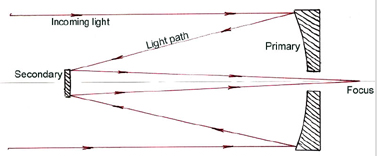
\includegraphics{cassegrain.png}
    \caption{Diagram showing the optical arrangement of the Cassegrain.}
    \label{cassegrain}
\end{figure}

The image will not necessarily be a perfect image: all rays regardless
of height at the surface (the lens or mirror),
$y$, might not cross at the same point. This
is the subject of aberrations, which we will get into in a while. For
a ``smooth'' surface, the amount of aberration will depend on how much
the different rays differ in $y$, which depends on the shape of the
surface. We define:
\begin{itemize*}
    \item \emph{paraxial} rays are near the center of the aperture.
    \item \emph{marginal} rays are on the edge of the aperture.
    \item the \emph{chief} ray passes through the center of the aperture.
\end{itemize*}
To define nominal (unaberrated) quantities, we consider the
\emph{paraxial regime}, a small region near the optical axis surrounding the
chief ray. In this regime, all angles are small, aberrations vanish,
and a surface can be wholly specified by its radius of curvature, $R$.

The \emph{field angle} (FA) gives the angle formed between the chief ray from an
object and the z-axis. Note that paraxial does not necessarily mean a
field angle of zero; one can have an object at a field angle and
still consider the paraxial approximation.

For the time being, we are ignoring \emph{diffraction}
and considering \emph{geometric} optics,
(what you get from diffraction as wavelength tends to 0).
For nonzero wavelength, geometric optics applies as scales
$x$ $>$ $\sim\lambda$.

We can derive the basic relation between the object location at $s$ and
the image location at $s'$ as a function of a surface where the index of
refraction changes (Schroeder, chapter 2).
$$  \frac{n'}{s'}-\frac{n}{s} = \frac{(n'-n)}{R}  $$
The points at $s$ and $s'$ are called \emph{conjugate}. If either $s$
or $s'$ is at infinity (true for astronomical sources at $s$), the
other distance is defined as the \emph{focal length}, $f$, of the
optical element. For $s=\infty$, $f=s'$.

We can define the quantity on the right side of the equation, which
depends only on the surface parameters (not the image or object
locations), as the \emph{power}, $P$, of the surface:
    $$ P \equiv \frac{(n'-n)}{R} = \frac{n'}{f'} = \frac{n}{f} $$
We can make a similar derivation for the case of reflection:
    $$ \frac{1}{s'} + \frac{1}{s} = \frac{2}{R}  $$
This shows that the focal length for a mirror is given by $R/2$.

Note that one can treat reflection by considering refraction with
$n' = -n$, and get the same result:
$$  \frac{n'}{s'}+\frac{n'}{s} = \frac{(n'+n')}{R}  $$
The \emph{focal ratio} (or \emph{F-number}) is defined as
$$ f/ = \frac{f}{A}$$
where A is the aperture diameter and $f/$ denotes the focal ratio.
(Note that, for example, $f /10$ means a focal ratio of 10;
$f$ is not some variable being divided by 10).
The focal ratio gives the beam ``width''; systems with a small focal ratio
have a short focal length compared with $A$, and hence the imcoming
beam to the image is wide. Systems with small focal ratios are called
``fast'' systems; systems with large focal ratios are called ``slow'' systems.
%--------------------------------------------------------------------%
\textcolor{magenta}{Wednesday, March 2}

The \emph{magnification} of a system gives the ratio of the image height to
the object height:
    $$  \frac{h'}{h} = \frac{s'-R}{s-R} = \frac{ns'}{n's}    $$
The magnification is negative for inverted images, and also for
reflection ($n' = -n$).
Magnification is an important quantity for \emph{multi-element} systems.

The \emph{plate scale} is defined as the
``motion'' of an image for a given incident angle
of parallel beam from infinity.
From a consideration of the chief rays
for objects on-axis and at field angle $ \alpha$, we get:
$$ \tan{\alpha} \approx \alpha = \frac{x}{f}  $$
or
$$ \textrm{scale} \equiv \frac{\alpha}{x} = \frac{1}{f}  $$
In other words, the scale, in units of angular motion per physical
motion in the focal plane, is given by $1/f$. For a fixed aperture
diameter, systems with a small focal ratio (smaller focal length) have
a larger scale, i.e.\ more light in a patch of fixed physical size:
hence, these are ``faster'' systems.

\subsection*{Multi-surface systems}
To combine surfaces, the image from the first surface becomes the
source for the second surface, and so on for each surface in the system.
The basic parameters of multi-surface systems can generally be described by
equivalent single-surface parameters.
For example, the effective focal length of a multi-surface system
can be defined as the focal length of some
equivalent single-surface system.
The \emph{effective} focal length is the
focal length of the first element multiplied by the magnification of
each subsequent element. The two systems (single and multi) are
equivalent in the paraxial approximation ONLY\@.

\subsubsection*{The two-surface lens}
Consider a lens in air ($n \sim 1$). The first surface gives:
    $$ \frac{n}{s_1'}-\frac{1}{s_1} = \frac{n-1}{R_1}=P_1  $$
The second surface gives:
    $$ \frac{1}{s_2'}-\frac{n}{s_2} = \frac{n-1}{R_2}=P_2  $$
but we have $s_2 = s_1'-d$ (remember we have to use the plane of the
second surface to measure distances for the second surface).

After some algebra, we find the effective focal length (from center of
lens):

    $$ P=\frac{1}{f'}=P_{1}+P_{2}-\frac{d}{n}P_{1}P_{2}   $$
    $$ P=\frac{(n-1)}{R_{1}}+\frac{(1-n)}{R_{2}}-\frac{d}{n}
         \frac{(n-1)(1-n)}{R_{1}R_{2}}  $$

From this, we derive the \emph{thin lens} formula:

    $$ P=\frac{1}{f'} = \frac{(n-1)}{R_{1}}+\frac{(1-n)}{R_{2}}
         = (n-1)\left( \frac{1}{R_1} - \frac{1}{R_2}\right)  $$
    $$ \frac{1}{f'} = \frac{1}{f_{1}} + \frac{1}{f_{2}}   $$

\subsubsection*{plane-parallel plate}
Zero power, but moves image laterally:
$$\Delta = d\left[1-\left(\frac{1}{n}\right)\right]$$
Application to filters: variation of focus.

\subsubsection*{Two-mirror telescopes}
In astronomy, most telescopes are two-mirror telescopes of Newtonian,
Cassegrain, or Gregorian design. All 3 types have a concave primary.
The Newtonian has a flat secondary, the Cassegrain a convex secondary,
and the Gregorian a concave secondary. The Cassegrain is the most
common for research astronomy; it is more compact than a Gregorian and
allows for magnification by the secondary. Basic parameters are
outlined
\href{http://astronomy.nmsu.edu/holtz/a535/html/diagrams/a535/cassegra.htm}
{\textcolor{blue}{here}}.
Each of these telescope types defines a \emph{family} of
telescopes with different first-order performances. From the
usage/instrumentation point of view, important quantities are:
\begin{itemize*}
    \item the diameter of the primary, which defines the light
        collecting power
    \item the scale of the telescope, which is related to the focal
        length of the primary and the magnification of the secondary:
        $$ f_{eff} = f_1m  $$
        (alternatively, the focal ratio of the telescope, which gives
        the effective focal length with the diameter)
    \item the back focal distance, which is the distance of the focal
        plane behind the telescope.
\end{itemize*}
From the design point of view, we need to specify:
\begin{itemize*}
    \item the radii of curvature of the mirrors
    \item the separation between the mirrors
\end{itemize*}
The relation between the usage and design parameters can be derived
from simple geometry. Some basic definitions:
\begin{itemize*}
    \item ratio of focal lengths, $\rho$:
        $$ \rho = \frac{R_2}{R_1} = \frac{f_2}{f_1}  $$
    \item magnification of the secondary, $m$ (be aware that $s_2'$ is
        negative for a Cassegrain):
        $$ m = -\frac{s_2'}{s_2} $$
    \item \emph{back focal distance},
        the distance from the primary vertex to
        the focal plane (often expressed in units of the primary focal
        length, or primary diameter):
        $$ f_{1}\beta = D\eta  $$
    \item primary focal ratio, $F1$:
        $$ F_{1} = \frac{f_{1}}{D} $$
    \item ratio of marginal ray heights, $k$ (directly related to
        separation of mirrors):
        $$ k = \frac{y_{2}}{y_{1}}  $$
\end{itemize*}
Using some geometry, we can derive some basic relations between these
quantities, in particular:
    $$ \rho = \frac{mk}{(m-1)}  $$
and
    $$ (1+\beta) = k(m+1)  $$
Usually, $f_1$ is limited by technology/cost. Then choose $m$ to match
desired scale. $k$ is related to separation of mirrors, and is a
compromise between making telescope shorter and blocking out more
light vs.\ longer and blocking less light; in either case,
the focal plane has to be kept behind the primary.

One final thing to note is how we focus a Cassegrain telescope. Most
instruments are placed at a fixed location behind the primary.
Ideally, this will be at the back focal distance, and everything
should be set as designed. However, sometimes the instrument may not
be exactly at the correct back focal distance, or it might move
slightly because of thermal expansion/contraction. In this case,
focussing is usually then done by moving the secondary mirror.

The amount of image motion for a given secondary motion is given by:
    $$ \frac{d\beta}{dk} = \frac{d}{dk}k(m+1)-1 $$
Working through the relations above, this gives:
    $$ \frac{d\beta}{dk} = m^{2}+1  $$
so the amount of focal plane motion ($f_{1}d\beta$) for a given amount
of secondary motion ($f_{1}dk$) depends on the magnification of the
system.

If you move the secondary you change $k$. Since $\rho$ is fixed by the
mirror shapes, it's also clear that you change the magnification as
you move the secondary; this is expected since you are changing the
system focal length, $f = mf_{1}$. So it's possible that a given
instrument could have a slightly varying scale if its position is not
perfectly fixed relative to the primary.

Note that even if the instrument is at exactly the back focal
distance, movement of the secondary is required to account for
mechanical changing of spacing between the primary and secondary as a
result of thermal expansion/contraction.

%------------------------------------------------------------------%
\subsubsection*{Definitions for multi-surface system: stops and pupils}
\textcolor{magenta}{Monday, March 7, 2016}
\begin{itemize*}
    \item aperture stop: determines the amount of light reaching an
        image (usually the primary mirror).
    \item field stop: determines the angular size of the field. This
        is usually the detector, but for a large enough detector, it
        could be the secondary.
    \item pupil: location where rays from all field angles fill the
        same aperture.
    \item entrance pupil: image of aperture stop as seen from source
        object (usually the primary).
    \item exit pupil: image of aperture stop formed by all subsequent
        optical elements.
\end{itemize*}
In a two-mirror telescope, the location of the exit pupil is where the
image of the primary is formed by the secondary. This can be calculated
using $s=d$ as the object distance (where $d$ is the separation of the
mirrors), then with the reflection equation, we can solve for $s'$
which gives the location of the exit pupil relative to the secondary
mirror. If one defines the quantity $\delta$, such that $f_1 \delta$
is the distance between the exit pupil and the focal plane,
then (algebra not shown):
$$ \delta = \frac{m^{2}k}{m+k-1} = \frac{m^{2}(1+\beta)}{m^{2}+\beta} $$
This pupil is generally not accessible, so if one needs access to a pupil,
additional optics are use.

The exit pupil is an important concept. When we discuss aberrations, it is
the total wavefront error at the exit pupil which gives the system aberration.
Pupils are important for aberration compensation. They can also be used to
put light at a location that is independent of pointing errors.
\subsection*{Aberrations}
\subsubsection*{Surface requirements for unaberrated images}
Next we consider non-paraxial rays. We first consider what surface is
required to make an unaberrated image.

We can derive the surface using Fermat's principle. Fermat's principle
states that light travels in the path such that infinitessimally small
variations in the path doesn't change the travel time to first order:
%{\Large$\frac{\textrm{d}t}{\textrm{d}l}$}
$\textrm{d}t/\textrm{d}l$
is a minimum.
For a single surface, this reduces to
the statement that light travels the path which takes the least time.
An alternate way of stating Fermat's principle is that the \emph{optical path
length} is unchanged to first order for a small change in path. The OPL
is given by:
$$ OPL = \int{c\textrm{d}t} = \int{\frac{c}{v}v\textrm{d}t} = \int{n\textrm{d}s}$$
Fermat's principle has a physical interpretation when one considers the
wave nature of light. It is clear that around a stationary point of the
optical path light, the maximum amount of light can be accumulated over
different paths with a minimum of destructive interference. By the wave
theory, light travels over all possible paths, but the light coming over
the ``wrong'' paths destructively interferes, and only the light coming over
the ``right'' path constructively interferes.

Fermat's principle can be used to derive the basic laws of reflection
and refraction (Snell's law).

Now consider a perfect imaging system that takes all rays from an object
and makes them all converge to an object. Since Fermat's principle says
the only paths taken will be those for which the OPL is minimally changed
for small changes in path, the only way a perfect image will be formed is
when all optical path lengths along a surface between an image and object
point are the same - otherwise the light doesn't get to this point.

Instead of using Fermat's principle, we could solve for the parameters
of a perfect surface using analytic geometry, but this would require an
inspired guess for the correct functional form of the surface.

We find that the perfect surface depends on the situation: whether the
light comes from a source at finite or infinite distance, and whether
the mirror is concave or convex. We consider the various cases now,
quoting the results without actually doing the geometry. In all cases,
consider the z-axis to be the optical axis, with the y-axis running
perpendicular. We want to know the shape of the surface, $y(z)$, that gives
a perfect image.

\textbf{\emph{Concave mirror with one conjugate at infinity}}

Sample application: primary mirror of telescope looking at stars.

Fermat's principle gives:
$$ y^{2} = 2R_{z} $$
where $R = 2f$, the radius of curvature at the mirror vertex. This equation
is that of a parabola. Note, however, that a prabola makes a perfect image
only for on-axis images (field angle = 0).

\textbf{\emph{Concave mirror with both conjugates at finite distances}}

Sample application: Gregorian secondary looking at image formed by primary.

For a concave mirror with both conjugates finite, we get an ellipse.
Again, this is perfect only for field angle = 0.
$$ \frac{(z-a)^2}{a^2} + \frac{y^2}{b^2} = 1 $$
$$ y^2 - \frac{2zb^2}{a} + \frac{z^2b^2}{a^2} = 0 $$
where
$$ a = \frac{s+s'}{2} $$
$$ b = \sqrt{(ss')} $$
$$ R = \frac{ss'}{s+s'} = \frac{2b^2}{a} $$

\textbf{\emph{Convex mirror with both conjugates at finite distance}}

Sample application: Cassegrain secondary looking at image formed by primary.

For a convex mirror with both conjugates finite, we get a hyperbola:
$$ \frac{(z-a)^2}{a^2} - \frac{y^2}{b^2} = 1 $$
$$ y^2 + \frac{2zb^2}{a} - \frac{z^2b^2}{a^2} = 0 $$
where
$$ a = \frac{s+s'}{2} $$
$$ b^2 = \sqrt{(-ss')} $$
($s$ is negative)
$$ R = -\frac{2b^2}{a} $$

\textbf{\emph{Convex mirror with one conjugate at infinity}}

For a convex mirror with one conjugate at infinity, we get a parabola.

\textbf{\emph{2D to 3D}}

Note that in all cases we've considered a one-dimension surface. We can
generalize to 2D surfaces by rotating around the z-axis; for the equations,
simply replace $y^2$ with $(x^2 + y^2)$.

\textbf{\emph{Conic sections}}

As you may recall from analytic geometry, all of these figures are
\emph{conic sections}, and it is possible to describe all of these figures with a
single equation:
$$ \rho^2 - 2R_z + (1+K)z^2 = 0 $$
where $ \rho^2 = x^2 + y^2 $
and $R$ is the radius of curvature at the mirror vertex,
$K$ is called the conic constant ($K = -e^2$, where $e$ is the eccentricity for
an ellipse, $e(b, a)$).
\begin{itemize*}
    \item $K > 0$ gives a prolate ellipsoid
    \item $K = 0$ gives a sphere
    \item $-1 < K < 0$ gives an oblate ellipsoid
    \item $K = - 1$ gives a paraboloid
    \item $K < - 1$ gives a hyperboloid
\end{itemize*}

%------------------------------------------------------------------%
\subsubsection*{Aberrations: general description and low-order aberrations}
\textcolor{magenta}{?, March ?, 2016}

Now consider what happens for surfaces that are not perfect, e.g. for
the cases considered above for $FA\neq 0$ (since only a sphere
is symmetric for all field angles), or for field angle 0 for a conic
surface which doesn't give a perfect image?

You get \emph{aberrations}; the light from all locations in the aperture
does not land at any common point.

One can consider aberrations in either of two ways:
\begin{itemize*}
    \item All rays don't land at a common point.
    \item Wavefront deviates from a spherical wavefront.
\end{itemize*}
These two descriptions are equivalent. The former refers to
\emph{transverse} aberrations, which give the distance by which the
rays miss the paraxial focus, or the \emph{angular} aberration, which is the
angle by which the rays deviate from the perfect ray which will hit
paraxial focus. For the latter, one discusses the wavefront error,
i.e., the deviation of the wavefront from a spherical wavefront as a
function of location in the exit pupil.

In general, the angular and transverse aberrations can be determined
from the optical path difference between a given ray and that of a
spherical wavefront. The relations are given by:
$$ \textrm{angular aberration}
= \frac{\textrm{d}2\Delta z}{\textrm{d}\rho}$$
$$ \textrm{transverse aberration}
= s'\frac{\textrm{d}\Delta z}{\textrm{d}\rho}$$
If the aberrations are not symmetric in the pupil, then
define angular and transverse $x$ and $y$ aberrations separately by taking
derivatives with respect to $x$ or $y$ instead of $\rho$.

\textbf{\emph{Spherical aberration}}

First, consider the axisymmetric case of looking at an object on axis
(field angle equal zero) with an optical element that is a conic
section. We can consider where rays land as $f(\rho)$, and derive
the effective focal length, $f_e(\rho)$, for an arbitrary conic
section:
%\begin{figure}
%    \includegraphics{spherical_ab.png}
%\end{figure}
$$ z_0 = \frac{\rho}{\tan(2\phi)} = \frac{\rho(1-(\tan\phi)^2)}{2\tan\phi}$$
$$ \tan\phi = \frac{\textrm{d}z}{\textrm{d}\rho} $$
from conic sections: \textcolor{red}{$\ldots$ a crapload of equations.}

Note that $f_e$ is independent of $z$ only for $K=-1$, a parabola.
Also note that $\Delta f$ is symmetric with respect to $\rho$.

We define spherical aberration as the aberration resulting from
$K\ne -1$. Rays from different radial positions in the entrance
aperture focus at different locations. It is an aberration which is
present on axis as seen
\href{http://astronomy.nmsu.edu/holtz/a535/html/diagrams/a535/spher.htm}
{\textcolor{blue}{here}}. Spherical aberration is symmetric in
the pupil. There is no location in space where all rays focus at a
point. Note that the behavior (image size) as a function of focal
position is not symmetric. One can define several criteria for where
the ``best focus'' might be, leading to the terminology paraxial
focus, marginal focus, diffraction focus, and the circle of least
confusion.

The asymmetric nature of spherical aberration as a function of focal
position distinguishes it from other aberrations and is a useful
diagnostic for whether a system has this aberration. This is shown in this
%\href{}
\textcolor{blue}{figure} which shows a sequence of images at different focal
positions in the presence of spherical aberration. We define
\emph{transverse spherical aberration} (TSA) as the image size at paraxial
focus. This is not the location of the minimum image size.
%\begin{figure}...

$$ \frac{\textrm{TSA}}{\Delta f} = \frac{\rho}{f-z(\rho)} $$
$$ \textrm{TSA} = 1(1+K)\frac{\rho^3}{2R^2} -
    3(1+K)(3+K)\frac{\rho^5}{8R^4} + \ldots $$
The difference in angle between the ``perfect'' ray from the parabola
and the actual ray is called the \emph{angular aberration}, in this case
\emph{angular spherical aberration} (ASA).
%\begin{figure}...
$$ \textrm{ASA} = 2(\phi_{P}-\phi) \approx \frac{d}{d\rho}(2\Delta z)
    \approx -(1+K)\frac{\rho^3}{R^3} $$
where $2\Delta z$ gives the optical path difference between the two rays.

This is simply related to the transverse aberration:
$$ \textrm{TSA} = \frac{R}{2}\textrm{ASA} $$
We can also consider aberration as the difference between our
wavefront and a spherical wavefront, which in this case is the
wavefront given by a parabolic surface.
%\begin{figure}...

$$ \Delta z = z_{\textrm{parabola}}-z(K) = -\frac{\rho^4}{8R^3}(1+K)+\ldots $$
This result can be generalized to any sort of aberration: the angular
and transverse aberrations can be determined from the optical path
difference between a given ray and that of a spherical wavefront. The
relations are given by:
$$ \textrm{angular aberration} = \frac{\textrm{d}(2\Delta z)}{d\rho} $$
$$ \textrm{transverse aberration} = s'\frac{\textrm{d}(2\Delta z)}{d\rho} $$
If the aberrations are not symmetric in the pupil, then we could
define angular and transverse $x$ and $y$ aberrations separation by taking
derivatives with respect to $x$ or $y$ instead of $\rho$.

\textbf{\emph{General aberration description}}

We can describe deviations from a spherical wavefront generally. Since
all we care about are optical path differences, we write an expression
for the optical path difference between an arbitrary ray and the chief
ray, and in doing this, we can also include the possibility of an
off-axis image, and get
$$ OPD = OPL - OPL(chiefray) $$
$$ OPD = A_0y + A_1y^2 + A_1'x^2 + A_2y^3 + A_2'x^2y + A_3\rho^4 $$
where we've kept terms only to fourth order and chosen our coordinate
system such that the object lies in the y-z plane. The coefficients,
$A$, depend on lots of things, such as ($\theta, K, n, R, s, s'$).

Note that rays along the y-axis are called \emph{tangential} rays,
while rays along the x-axis are called \emph{sagittal} rays.

Analytically, people generally restrict themselves to talking about
\emph{third-order} aberrations, which are fourth-order
(in powers of $x, y, \rho$, or $\theta$) in the optical path
difference, because of the derivative we take to get transverse or
angular aberrations. In the third-order limit, one finds that
$A2 = A2'$, and $A1 = -A1'$. Working
out the geometry, we find for a mirror that:
\textcolor{red}{Craploads more equations.}

$$ A_0 = 0 $$
$$ A_1 = \frac{n\theta^2}{R} $$
$$ A_2 = -\frac{n\theta}{R^2}\left(\frac{m+1}{m-1}\right) $$
$$ A_3 = \frac{n}{4R^3}\left[K+\left(\frac{M+1}{M-1}\right)^2 \right] $$

From the general expression, we can derive the angular or the
transverse aberrations in either the $x$ or $y$ direction. Considering the
aberrations in the two separate directions, we find:

$$ AA_y = 2A_1y + A_2(x^2+3y^2) + 4A_3y\rho^2  $$
$$ AA_x = 2A_1'x + 2A_2xy + 4A_3x\rho^2  $$

The first term is proportional to $\theta^{2}y$ and is called
\emph{astigmatism}. The second term is proportional to
$ \theta(x^2 +3y^2)$
and is called \emph{coma}. The final term, proportional to
$y\rho^{2}$
is \emph{spherical aberration}, which we've already discussed (note for
spherical, $AA_x = AA_y$ and in fact the $AA$ in any direction is equal,
hence the aberration is circularly symmetric).

\textbf{\emph{Astigmatism}}

For astigmatism, rays from opposite sides of the pupil focus in
different locations relative to the paraxial rays. At the paraxial
focus, we end up with a circular image. As you move away from this
image location, you move towards the tangential focus in one
direction and the sagittal focus in the other direction. At either of
these locations, the astigmatic image looks like a elongated ellipse.
Astigmatism goes as $\theta^{2}$, and consequently looks the same
for opposite field angles. Astigmatism is characterized in the image
plane by the \emph{transverse} or \emph{angular} astigmatism (TAS or AAS), which
refer to the height of the marginal rays at the paraxial focus.
Astigmatism is symmetric around zero field angle.

This \href{http://astronomy.nmsu.edu/holtz/a535/html/diagrams/a535/astig.htm}
{\textcolor{blue}{figure}} shows the rays in the presence of astigmatism.
This \href{http://astronomy.nmsu.edu/holtz/a535/html/diagrams/a535/z5.htm}
{\textcolor{blue}{figure}}
shows the behavior of astigmatism as one passes through paraxial focus.

\textbf{\emph{Coma}}

For coma, rays from opposite sides of the pupil focus at the same
focal distance. However, the tangential rays focus at a different
location than the sagittal rays, and neither of these focus at the
paraxial focus. The net effect is to make an image that vaguely looks
like a comet, hence the name coma. Coma goes as $\theta$, so the
direction of the comet flips sign for opposite field angles. Coma is
characterized by either the \emph{tangential} or \emph{sagittal
transverse/angular coma} (TTC, TSC, ATC, ASC) which describe the
height/angle of either the tangential or sagittal marginal rays at the
paraxial focus: $TTC = 3TSC$.

This \href{http://astronomy.nmsu.edu/holtz/a535/html/diagrams/a535/coma.htm}
{\textcolor{blue}{figure}} shows the rays in the presence of coma.
This \href{http://astronomy.nmsu.edu/holtz/a535/html/diagrams/a535/z7.htm}
{\textcolor{blue}{figure}} shows the behavior of coma as one passes
through paraxial focus.
In fact, there are two more third-order aberrations:
\emph{distortion} and \emph{field curvature}.
Neither affects image quality, only location (unless
you are forced to use a flat image plane). Field curvature gives a
curved focal plane: if imaging onto a flat detector, this will lead to
focus deviations as one goes off-axis. Distortion affects the location
of images in the focal plance, and goes as $\theta^{3}$.
The amount of field curvature and distortion can be derived from the
aberration coefficients and the mirror parameters.

We can also determine the relevant coefficients for a surface with a
displaced stop (Schroeder p 77), or for a surface with a decentered
pupil (Schroeder p89-90); it's just more geometry and algebra. With
all these realtions, we can determine the optical path differences for
an entire system: for a multi-surface system, we just add the OPD's as
we go from surface to surface. The final aberrations can be determined
from the system OPD.

\subsubsection*{Aberration compensation and different telescope types}
\textcolor{magenta}{Wednesday, March 30}

Using the techniques above, we can write expressions for the system
aberrations as a function of the surface figures (and field angles).
If we give ourselves the freedom to choose surface figures, we can
eliminate one (or more) aberrations.

For example, given a conic constant of the primary mirror, we can use
the aberration relations to determine $K_2$ such that spherical
aberration is zero; this will give us perfect images on-axis. We find
that:
$$ K_2 = \left(\frac{m+1}{m-1}\right)^2 +
    \frac{m^{3}}{k\left(m-1\right)^{3}}\left(K_{1}+1\right) $$
satisfies this criterion.  If we set the primary to be a parabola
($K_{1} = -1$), this gives the conic constant of the secondary we must use to
avoid spherical aberration. This type of telescope is called a
\emph{classical} telescope. Using the aberration relations, we can determine
the amount of astigmatism and coma for such telescopes, and we find
that coma gives significantly larger aberrations than astigmatism.

If we allow ourselves the freedom to choose both $K_1$ and $K_2$,
we can eliminate both spherical aberration and coma.
Designs of this sort are called \emph{aplanatic}.
The relevant expression, in terms of the magnification and
back focal distance (we could use the relations discussed earlier to
present these in terms of other paraxial parameters), is:
$$ K_{1} = -1 - \frac{2(1+\beta)}{m^{2}(m-\beta)} $$
We can only eliminate two aberrations with two mirrors, so even this
telescope will be left with astigmatism.

There are two different classes of two-mirror telescopes that allow
for freedom in the shape of both mirrors: Cassegrain telescopes and
Gregorian telescopes (Newtonians have a flat secondary). For the
classical telescope with a parabolic primary, the Cassegrain
secondary is hyperbolic, whereas for a Gregorian it is ellipsoidal
(because of the appropriate conic sections derived above for convex
and concave mirrors with finite conjugates). For the aplanatic
design, the Cassegrain telescope has two hyperbolic mirrors, while
the Gregorian telescope has two ellipsoidal mirrors. An aplanatic
Cassegrain telescope is called a \emph{Ritchey-Chretien} telescope.

The following table gives some characteristics of ``typical''
telescopes. Aberrations are given at a field angle of 18 arc-min in
units of arc-seconds. Coma is given in terms of tangential coma.

\begin{table}[h]
\centering
\begin{tabular}{c r r r r}
Parameter & CC & CG & RC & AG\\
\hline\hline
m & 4.00 & -4.00 & 4.00 & -4.00\\
k & 0.25 & -0.417 & 0.25 & -0.417\\
1-k & 0.75 & 1.417 & 0.75 & 1.417\\
mk & 1.000 & 1.667 & 1.000 & 1.667\\
ATC & 2.03 & 2.03 & 0.00 & 0.00\\
AAS & 0.92 & 0.92 & 1.03 & 0.80\\
ADI & 0.079 & 0.061 & 0.075 & 0.056\\
$\kappa_{m}R_{1}$ & 7.25 & -4.75 & 7.625 & -5.175\\
$\kappa_{P}R_{1}$ & 4.00 & -8.00 & 4.00 & -8.00\\
\hline
\end{tabular}
\caption{Characteristics of Two-Mirror Telescopes}
\end{table}

The image quality is clearly better for the aplanatic designs than for
the classical designs, as expected because coma dominates off-axis in
the classical design. In the aplanatic design, the Gregorian is
slightly better. However, when considerations other than just optical
quality are considered, the Cassegrain usually is favored: for the
same primary mirror, the Cassegrain is considerably shorter and thus
it is less costly to build an enclosure and telescope structure. To
keep the physical length the same, the Gregorian would have to have a
faster primary mirror, which are more difficult (i.e. costly) to
fabricate, and which will result in a greater sensitivity to alignment
errors. Both types of telescopes have a \emph{curved} focal plane.

\subsection*{Sources of aberrations}
So far, we have been discussing aberrations which arise from the
optical design of a system when we have a limited number of elements.
However, it is important to realize that aberrations can arise from
other sources as well. These other sources can give additional
third-order aberrations, as well as higher order aberrations. Some
possible sources include:
\begin{itemize*}
    \item misfigured (a slightly harsh term)
        or imperfectly figured optics: rarely is an element made
        exactly to specification.
    \item misalignments. If the mirrors in a multiple-element system are not
        perfectly aligned, aberrations will result. The centers must be
        lined up.  These can be derived
        (third-order) from the aberration expressions for decentered elements.
        For two mirror systems, decentering or tilting the
        secondary introduces a constant amount of coma over the field. Coma
        dominates astigmatism for a misaligned telescope.
        The Ritchey-Chretian has a ``high'' tolerance for this (not much
        wiggle room).
    \item mechanical/support problems. When the mirrors are mounted in mirror
        cells the weight of the mirror is distributed over some support
        structures. Because the mirrors are not infinitely stiff, some
        distortion of the mirror shape will occur. Generally, such distortion
        will probably change as a function of which way the telescope is
        pointing. Separate from this, becuase the telescope structure itself
        is not perfectly stiff, one expects some flexure which gives a
        different secondary (mis)alignment as a function of where one is
        pointing. Finally, one might expect the spacing between the primary
        and secondary to vary with temperature, if the telescope structure is
        made of materials which have non-zero coefficients of expansion.
    \item chromatic aberration. Generally, we've only been discussing mirrors
        since this is what is used in telescopes. However, astronomers often
        put additional optics (e.g., cameras or spectrographs) behind
        telescopes which may use refractive elements rather than mirrors.
        There are aberration relations for refractive elements just as we've
        discussed, but these have additional dependences on the indices of
        refraction of the optical elements. For most refractive elements, the
        index of refraction varies with wavelength, so one will get
        wavelength-dependent aberrations, called chromatic aberrations. These
        can be minimized by good choices of materials or by using combinations
        of different materials for different elements; however, it is an
        additional source of aberration.
    \item seeing. This is the only natural source of aberration (the one
        we can't control).
        The earth's atmosphere introduces optical path differences
        between the rays across the aperture of the telescope. This is
        generally the \textbf{dominant} source of image degradation from a ground-based
        telescope. Consequently, one builds telescopes in good sites, and as
        far as design and other sources of image degradation are concerned,
        one is generally only interested in getting these errors small when
        compared with the smallest expected seeing errors.
\end{itemize*}

\subsection*{Ray tracing}

For a fully general calculation of image quality, one does not wish
to be limited to third-order aberrations, nor does one often wish to
work out all of the relations for the complex set of aberrations
which result from all of the sources of aberration mentioned above.
Real world situations also have to deal with \emph{vignetting} in optical
systems, in which certain rays may be blocked by something and never
reach the image plane (e.g., in a two-mirror telescope, the central
rays are blocked by the secondary).

Because of these and other considerations, analysis of optical
systems is usually done using \emph{ray tracing}, in which the parameters of
an optical system are entered into a computer, and the computer
calculates the expected images on the basis of geometric optics. Many
programs exist with many features: one can produce \emph{spot} diagrams
which show the location of rays from across the aperture at an image
plane (or any other location), plots of transverse aberrations, plots
of optical path differences, etc. \texttt{zmacs} is a ray-tracing
program.

(Demo ray trace program. Start with on-axis object, single mirror.
Where is focus? What will image look like with spherical mirror? What
do we need to do to make it perfect? How does it depend on aperture
size? Now how do off-axis images look like? spot diagrams, through
focus, ray fan, opd plots, etc. Now introduce second mirror. What
determines where focus will be? Magnification? What shape to make a
perfect on-axis image? What do off-axis images look like? How do we
make them better? Now how is performance? Real 3.5m and 1m
prescriptions. Issue: guider.)

\subsection*{Physical (diffraction) optics}

Up until now, we have avoided considering the wave nature of light
which introduces \emph{diffraction} from interference of light coming from
different parts of the aperture. Because of diffraction, images of a
point source will be slightly blurred. From simple geometric arguments,
we can estimate the size of the blur introduced from diffraction:
%\begin{figure}...

We find that:
$$ \theta \sim \frac{\lambda}{D}  $$

Using this, we find that the diffraction blur is smaller than the blur
introduced by seeing for $D > 0.2$ meters at 5500 \AA{}, even for the
excellent seeing conditions of 0.5 arcsecond images. However, the
study of diffraction has become important recently because of several
reasons: 1) the existence of the Hubble Space Telescope, which is
diffraction limited (no seeing), 2) the increasing use of infrared
observations, where diffraction is more important than in the optical,
and 3) the development of adaptive optics, which attempts to remove
some of the distortions caused by seeing. Consequently, it's now
worthwhile to understand some details about diffraction.

To work out in detail the shape of the images formed from diffraction
involves understanding wave propagation. Basically, one integrates
over all of the source points in the aperture (or exit pupil for an
optical system), determining the contribution of each point at each
place in the image plane. The contributions are all summed taking into
account phase differences at each image point, which causes
reinforcment at some points and cancellation at others. The expression
which sums all of the individual source points is called the
\emph{diffraction integral}. When the details are worked out,
the intensity in the image plane is related to the intensity and phase
at the exit pupil. In fact the wavefront is described at any plane by
the \emph{optical transfer function}, which gives the intensity and phase of
the wave at all locations in that plane. The OTF at the pupil plane
and at the image plane are a Fourier transform pair. Consequently, we
can determine the light distribution in the image plane by taking the
Fourier transform of the pupil plane; the light distribution, or point
spread function, is just the modulus-squared of the OTF at the image
plane. Symbolically, we have

$$ PSF = \left\vert FT(OTF(pupil))\right\vert^2 $$

where $FT$ represents a Fourier transform, and

$$ OTF(pupil) = P(x,y)\exp{ik\phi(x,y)} $$

$P(x,y)$ is the \emph{pupil function}, which gives the transmission
properties of the pupil, and usually consists of ones and zeros for
locations where light is either transmitted or blocked (e.g., for a
circular lens, the pupil function is unity within the radius of lens,
and zero outside; for a typical telescope the pupil function includes
obscuration by the secondary and secondary support structure).
$\phi$ is the phase in the pupil. More relevantly, $\phi$ can be
taken to be the optical path difference in the pupil with some
fiducial phase, since only OPDs matter, not the absolute phase.
Finally the wavenumber $k$ is just $\frac{2\pi}{\lambda}$.

For the simple case of a plane wave with no phase errors, the
diffraction integral can be solved analytically. The result for a
circular aperture with a central obscuration, when the fractional
radius of the obscuration is given by $\epsilon$, the expression for
the PSF is:

$$ PSF \propto \left[\frac{2J_1(v)}{v}-
    \epsilon^2\frac{2J_1(\epsilon v)}{\epsilon v} \right]^2$$

    $$ v = \frac{\pi r}{\lambda F} $$

where $J_1$ is a first order Bessel function, $r$ is the distance in the
image plane, $\lambda$ is the wavelength, and $F$ is the focal ratio
($F=f/D$).

This expression gives the so-called \emph{Airy pattern} (the solution?)
which has a central disk surrounded by concentric dark and bright rings.
The radius of the first dark ring is at the physical distance
$r = 1.22\lambda F$, or alternatively, the angular distance
$\alpha = 1.22\lambda/D$. This gives the size of the \emph{Airy disk}.

For more complex cases, the diffraction integral is solved
numerically by doing a Fourier transform. The pupil function is often
more complex than a simple circle, because there are often additional
items which block light in the pupil, such as the support structures
for the secondary mirror.

This \href{http://astronomy.nmsu.edu/holtz/a535/html/diagrams/a535/airy.htm}
{\textcolor{blue}{figure}} shows the Airy pattern, both without obscurations,
and with a central obscuration and spiders in a setup typical of a telescope.

In addition, there may be phase errors in the exit pupil, because of
the existence of any one of the sources of aberration discussed
above. For general use, $\phi$ is often expressed as an series,
where the expansion is over a set of orthogonal polynomials for the
aperture which is being used. For circular apertures with (or
without) a central obscuration (the case most often found in
astronomy), the appropriate polynomials are called \emph{Zernike}
polynomials. The lowest order terms are just uniform slopes of phase
across the pupil, called tilt, and simply correspond to motion in the
image plane. The next terms correspond to the expressions for the OPD
which we found above for focus, astigmatism, coma, and spherical
aberration, generalized to allow any orientation of the phase errors
in the pupil. Higher order terms correspond to higher order
aberrations.

This \href{http://astronomy.nmsu.edu/holtz/a535/html/diagrams/a535/zernike.htm}
{\textcolor{blue}{figure}} shows the form of some of the low order Zernike terms:
the first corresponds to focus aberration, the next two to
astigmatism, the next two to coma, the next two to trefoil
aberration, and the last to spherical aberration.

A wonderful example of the application of all of this stuff was in the
diagnosis of spherical aberration in the Hubble Space Telescope, which
has been corrected in subsequent instruments in the telescope, which
introduce spherical aberration of the opposite sign. To perform this
correction, however, required and accurate understanding of the
amplitude of the aberration. This was derived from analysis of
on-orbit images, as shown in this
\href{http://astronomy.nmsu.edu/holtz/a535/html/diagrams/a535/hstspher.htm}
{\textcolor{blue}{figure}}. Note that it is possible in
some cases to try to recover the phase errors from analysis of images.
This is called phase retrieval. There are several ways of trying to do
this, some of which are complex, so we won't go into them, but it's
good to know that it is possible. But an accurate amplitude of
spherical aberration was derived from these images. This derived value
was later found to correspond almost exactly to the error expected
from an error which was made in the testing facility for the HST
primary mirror, and the agreement of these two values allowed the
construction of new corrective optics to proceed$\ldots$

\subsection*{Adaptive optics}
\textcolor{magenta}{Monday, April 4}

%------------------------------------------------------------------%















\end{document}
